\documentclass[a4paper, 10.5pt]{article}

\usepackage[italian]{babel}
\usepackage[utf8]{inputenc}
\usepackage{subfig}
\usepackage{siunitx}
\usepackage{geometry}
\usepackage{graphicx}
\usepackage{caption}
\usepackage{float}
\usepackage{array}
\usepackage{wrapfig}
\usepackage{amsfonts}
\usepackage{multirow}
\usepackage{siunitx}
\usepackage{color, colortbl}
\definecolor{Gray}{gray}{0.9}
\sisetup{round-mode = places, round-precision = 2, table-parse-only}
\geometry{a4paper, top=2.5cm, bottom=2.5cm, left=2.7cm, right=2.7cm}
\newcolumntype{P}[1]{>{\centering\arraybackslash}p{#1}}
\newcolumntype{M}[1]{>{\centering\arraybackslash}m{#1}}
\captionsetup{labelfont=bf, justification=centering}
\sisetup{round-mode = figures,round-precision = 3}
\includeonly{DataUnderstanding, clustering, AssociationRules, Classification, Conclusioni}


\begin{document}
    \begin{titlepage}

        \newcommand{\HRule}{\rule{\linewidth}{0.5mm}}

        \center % Center everything on the page
        
        
\includegraphics[width = 0.25\textwidth]{prima_pg/unipi.png}\\
        \hspace*{\fill}
        
        \textsc{\LARGE Università di Pisa}\\[1.5cm] %
        \textsc{\Large }\\[0.5cm] 
        \textsc{\LARGE \textit {Data Mining project}}\\[0.8cm]
        \HRule \\[0.8cm]
        { \huge \bfseries Perché i lavoratori lasciano un'azienda?}\\[0.4cm]
        \LARGE\textbf{ Il caso IBM}
        
        \HRule \\[1.5cm]
        \textsc{\Large\textit{{A cura di\\Erica Cau, Alfonso Ferraro, Simona Mazzarino, Federico Mazzoni}}}
  
%----------------------------------------------------------------------------------------

    \end{titlepage}
    
    \section{Introduzione}
Il \textit{dataset}\textit{ IBM HR }è una raccolta di dati creata da IBM (\textit{International Business Machine Corporation}), azienda americana leader nel settore informatico, per studiare le ragioni che portano i propri dipendenti all'autolicenziamento. L'obiettivo della seguente indagine è dunque quello di analizzare il dataset per comprendere quali siano le variabili che più frequentemente influenzano la suddetta scelta.
\\\\
Il progetto è suddiviso in quattro sezioni: \textit{Data Understanding, Clustering}, \textit{Classification} e \textit{Association Rules Mining}. Nel paragrafo dedicato al \textit{Data Understanding} prepareremo il dataset attraverso la \textit{Data Semantics}, la distribuzione statistica dei dati, la \textit{Data Quality} e infine la pulizia dei dati stessi. 
\\\\
Le parti successive saranno destinate all'esplorazione del dataset e alla comprensione del fenomeno dell'abbandono del posto di lavoro per mezzo di algoritmi di \textit{clustering, association rules mining} e \textit{classification}. L'ultima sezione sarà invece riservata alle considerazioni finali.
\section{Data Understanding}
%Tabella attributi categorici
\begin{table}[H]
\resizebox{0.99\textwidth}{!}{
%\centering
\begin{tabular}{ |p{4cm}|p{3cm}|}
 \hline
 \multicolumn{2}{|c|}{\textbf{Categorici}} \\
 \hline
 \textbf{Ordinali}     & \textbf{Nominali} \\
 \hline
 Education & Attrition\\
 EnvironmentSatisfation & BusinessTravel \\
 JobInvolvement & Department\\
 JobSatisfaction & EducationField\\
 PerformanceRating & Gender\\
 RelationshipSatisfaction & JobRole\\
 WorkLifeBalance & MaritalStatus\\
 StockOptionLevel   & Over18\\
 JobLevel & OverTime\\
 &\\
 &\\
 &\\
\hline
\end{tabular}
\quad
%Tabella attributi numerici
\begin{tabular}{ |p{4.6cm}|p{2.7cm}|}
 \hline
 \multicolumn{2}{|c|}{\textbf{Numerici}} \\
 \hline
 \textbf{Continui}     & \textbf{Discreti} \\
 \hline
  Age  & DailyRate  \\
  TotalWorkingYears & MonthlyRate \\
  Hourly Rate & MonthlyIncome \\
  YearsAtCompany& \\
  DistanceFromHome& \\
NumCompaniesWorked & \\
PercentSalaryHike& \\
StandardHours&\\
TrainingTimeLastYear&\\
YearsInCurrentRole&\\
YearsSinceLastPromotion&\\
YearsWithCurrentManager&\\
 \hline
\end{tabular}
}
\caption{\textit{Attributi categorici e numerici nel dataset}}
 \label{TabellaAttributiCatNum}
\end{table}
% df.describe(), inserire informazioni generali sul dataset
Il dataset IBM HR è formato da \textit{1176 record} (o oggetti) e \textit{33 \textit{feature}} (o attributi) di cui 18 categoriche e 15 numeriche. All'interno della colonna degli attributi nominali, nella tabella \ref{TabellaAttributiCatNum}, alcune variabili, nello specifico \textit{Attrition, Gender, Over18, OverTime}, sono classificate come binarie. L'attributo \textit{Over18} presenta, inoltre, la caratteristica di possedere i seguenti valori: "Y", interpretato come \textit{Yes} e valore "NaN".

\subsection{Data semantic}
Tra le \textit{\textit{feature}} più interessanti del dataset, figura sicuramente l'attributo binario \textit{Attrition}, ovvero il tasso di abbandono della posizione lavorativa dalla IBM, a cui sono associati due valori: \textit{Yes} e \textit{No}. \\\\Ad essa si ricollegano altri attributi volti a indagare il livello d’istruzione dei dipendenti, il loro campo di studi (\textit{Education} e \textit{EducationField}), il ruolo all’interno dell’azienda (\textit{JobRole}) e il livello delle performance lavorative (\textit{PerformanceRating}). Viene anche posta attenzione al tempo destinato alla formazione aziendale, agli anni di impiego sotto lo stesso manager (\textit{YearsWithCurrentManager}) e agli anni nel ruolo attuale ({\textit{YearsInCurrentRole}}). \\\\Per ogni impiegato sono inoltre valutate diverse sfumature di soddisfazione, legate sia al rapporto con l’azienda che con il lavoro in sé (\textit{JobSatisfaction} e \textit{RelationshipSatisfaction}), sia rispetto all'ambiente lavorativo (\textit{EnvironmentSatisfaction}).
\begin{table}
\centering
\large
\begin{tabular}{ |p{6.5cm}|p{8cm}|}
\hline
 \textbf{\textit{feature}} & \textbf{Descrizione} \\
 \hline
Age, Over18 & Età dei dipendenti e maggiore età \\
\hline
 Attrition & Abbandono della posizione lavorativa\\
\hline
BusinessTravel & Viaggi di lavoro\\
\hline
HourlyRate, DailyRate, MonthlyRate & Tariffa oraria, giornaliera e mensile\\
\hline
Department & Reparto aziendale di lavoro \\
\hline
DistanceFromHome& Distanza in KM dal domicilio\\
\hline
Education, EducationField & Livello d'istruzione e ambito di studi \\
\hline
EnvironmentSatisfaction& Gradimento dell'ambiente lavorativo misurato in scala numerica\\
\hline
Gender& Sesso del dipendente\\
\hline
JobInvolvement& Coinvolgimento nel lavoro misurato in scala numerica \\
\hline
JobLevel& Livello della posizione lavorativa misurato in scala numerica \\
\hline
JobSatisfaction& Gradimento del lavoro misurato in scala numerica\\
\hline
JobRole& Posizione lavorativa\\
\hline
MaritalStatus & Stato civile\\
\hline
MonthlyIncome, PercentSalaryHike& Stipendio mensile e Aumento salariale in percentuale \\
\hline
NumCompaniesWorked& Numero di aziende in cui il dipendente ha lavorato precedentemente\\
\hline
PerformanceRating& Valutazione delle prestazioni misurata in scala numerica\\
\hline
RelationshipSatisfaction& Gradimento del rapporto tra dipendente e azienda\\
\hline
StockOptionLevel& Piani di \textit{Stock Option} offerti dall'azienda ai dipendenti come incentivo \\
\hline
TotalWorkingYears& Totale degli anni in cui il dipendente ha lavorato nel corso della sua vita\\
\hline
StandardHours, OverTime& Totale delle ore lavorative contrattuali e straordinari\\
\hline
TrainingTimeLastYear& Periodo di formazione nell'ultimo anno\\
\hline
WorklifeBilance & Equilibrio tra lavoro e vita privata misurato in scala numerica\\
\hline
YearsAtCompany & Anni di impiego alla IBM\\
\hline
YearsInCurrentRole& Totale degli anni in cui il dipendente ricopre la stessa posizione lavorativa\\
\hline
YearsSinceLastPromotion&Totale degli anni trascorsi dall'ultima promozione\\
\hline
YearsWithCurrentManager& Totale degli anni trascorsi sotto lo stesso dirigente \\
 \hline
\end{tabular}
\caption{\textit{Descrizione degli attributi del dataset}}
\label{Descrizionefeature}
\end{table}

\subsection{Distribuzione statistica delle \textit{\textit{feature}}}
In questa sezione ci dedicheremo a un'analisi più approfondita delle distribuzioni statistiche delle \textit{\textit{feature}} più rilevanti, studiandole sia individualmente sia in correlazione tra loro, mentre in seguito discuteremo brevemente i risultati delle operazioni statistiche applicate alle \textit{\textit{feature}} categoriche e numeriche.
\begin{wrapfigure}{r}{0.49\textwidth}
\centering
    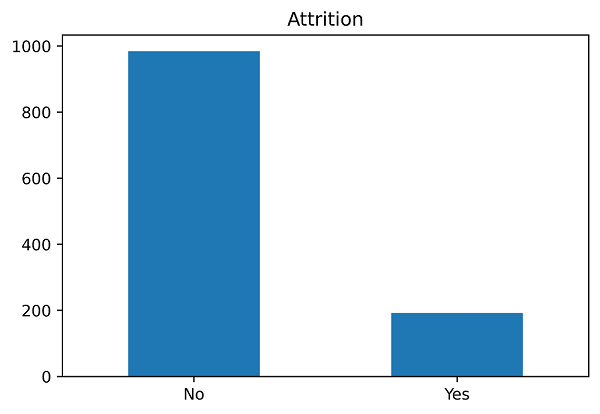
\includegraphics[width=0.46\textwidth]{Immagini/Grafico_Attrition.png}
    \setlength{\belowcaptionskip}{-10pt}
    \caption{Distribuzione della \textit{\textit{feature} Attrition}}
    \label{GraficoAttrition}
\end{wrapfigure}
\\\\\textbf{\textit{Attrition}}, la \textit{\textit{feature}} binaria da cui tutta la nostra analisi è partita, può assumere i valori \textit{Yes} e \textit{No}. Come si può osservare nella figura \ref{GraficoAttrition} la distribuzione è fortemente sbilanciata: è molto più elevato il numero di dipendenti che rimangono in azienda (83,67\% sul totale) rispetto a quelli che decidono di lasciarla (16,33\%). Una prima intuizione ci ha portato a correlarla con lo stipendio mensile (\textit{MonthlyIncome}) e con il numero totale degli anni trascorsi dall'ultima promozione \textit{YearsSinceLastPromotion}.
\\\\\\
\textbf{\textit{MonthlyIncome}}, lo stipendio mensile di ogni lavoratore, come possiamo vedere in figura \ref{DistrMonthlyIncome}, ha una distruzione sbilanciata verso i valori bassi. Risulta quindi un numero molto elevato di lavoratori che percepisce uno stipendio in un range che va dai 2500\$ ai 7500\$ e un numero considerevolmente più basso di lavoratori con stipendi medio-alti rispetto ai valori presenti nel dataset. È tuttavia presente un leggero aumento nella fascia di dipendenti che percepiscono una paga mensile compresa tra 17000\$ e 20000\$.
\begin{figure}[H]
	\centering
	\subfloat[]
	{
		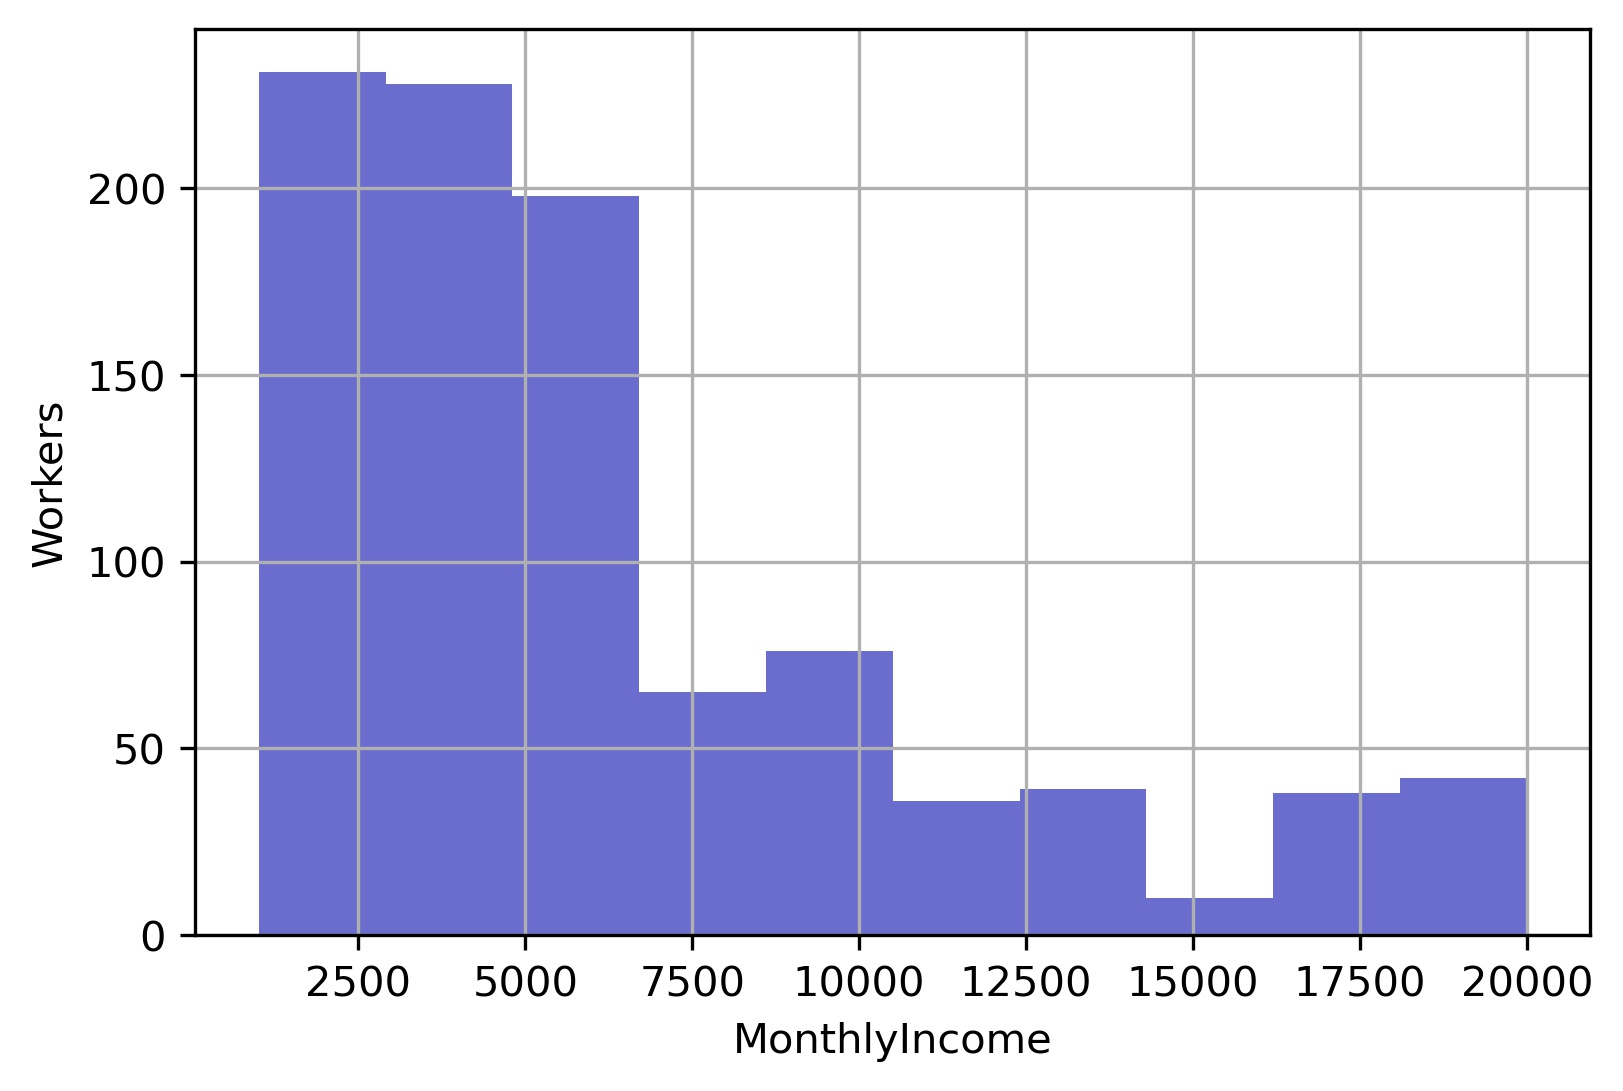
\includegraphics[width =0.45\textwidth]{Immagini/MonthlyIncome.jpeg}
		\label{DistrMonthlyIncome}
	}
	\quad
	\subfloat[]
	{
		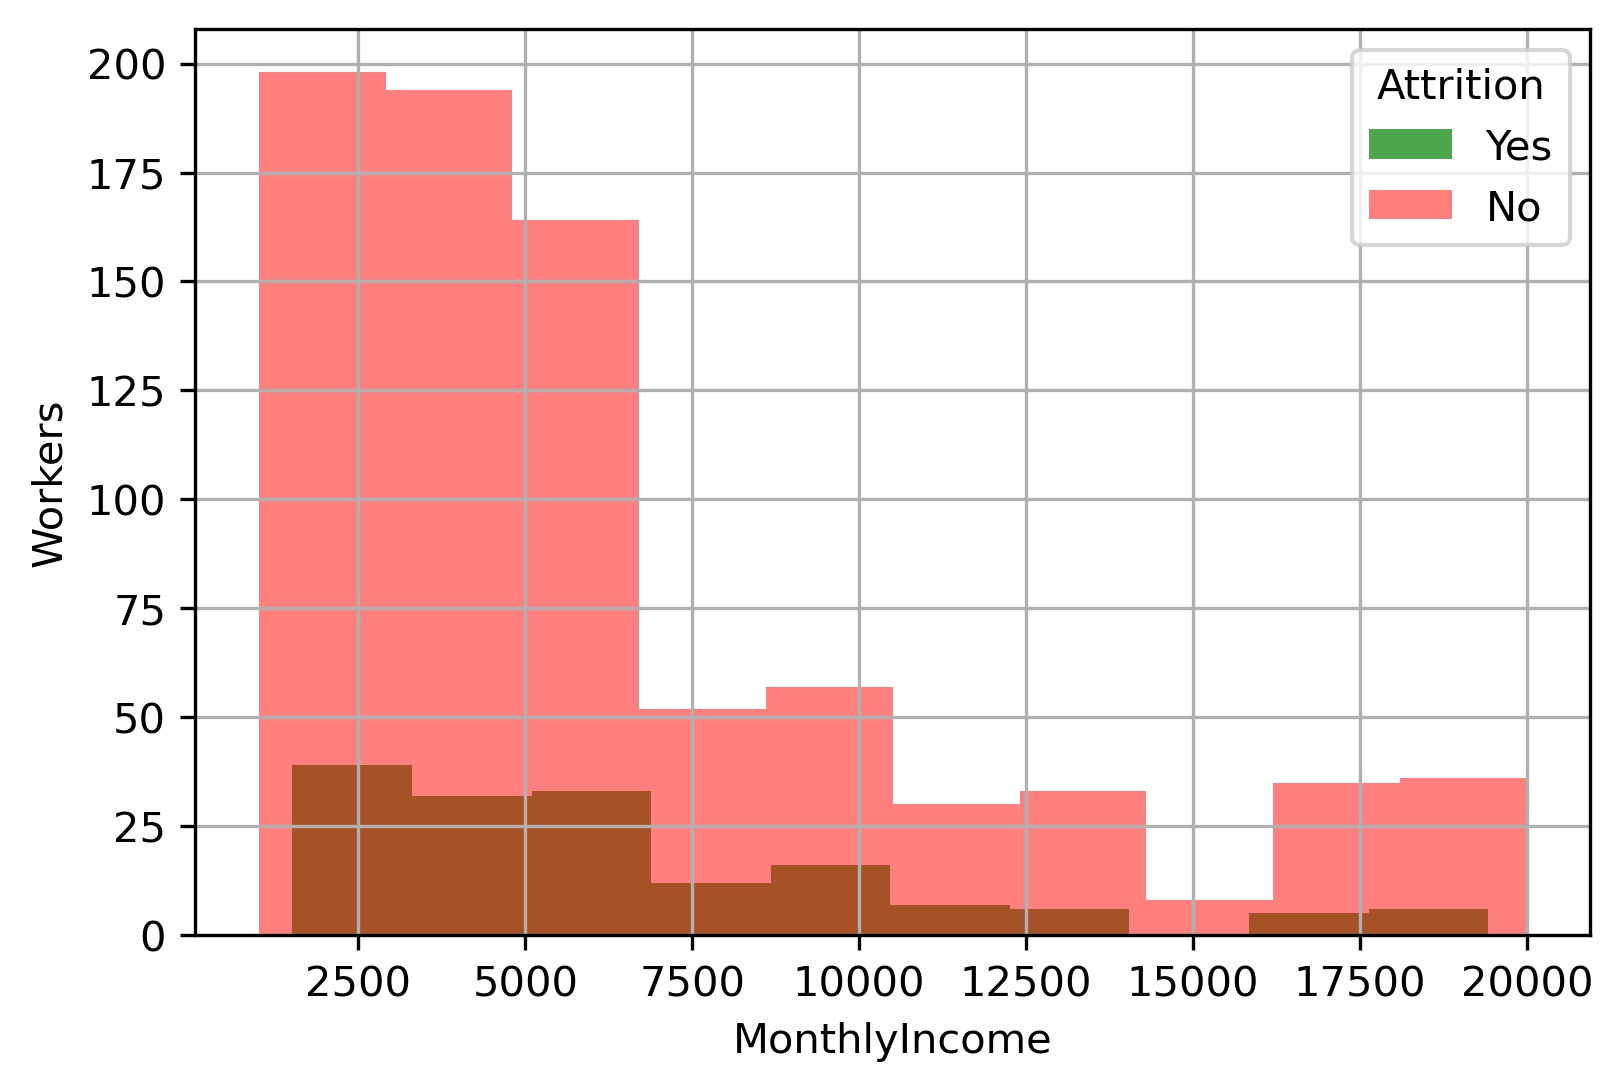
\includegraphics[width=0.45\textwidth]{Immagini/Attrition_MonthlyIncome1.jpeg}
		\label{AttrMonthlyIncome}
	}
	\caption{Distribuzione statistica dello stipendio mensile e del tasso di \textit{Attrition} in base allo stipendio}
	\label{GraficiStipendio}
\end{figure}
\noindent Come rappresentato in figura \ref{AttrMonthlyIncome}, la maggior parte delle persone che hanno deciso di lasciare il proprio posto di lavoro otteneva a fine mese uno stipendio compreso in un range basso. Tuttavia, anche in questo grafico, come in quello precedente, si nota un lieve incremento di \textit{Attrition} in corrispondenza di stipendi elevati: in questo contesto, si può ipotizzare che la crescita dei valori positivi di \textit{Attrition} sia dovuta a possibili pensionamenti.
\\\\
\textbf{\textit{YearsSinceLastPromotion}} è la \textit{\textit{feature}} che descrive gli anni trascorsi dall'ultima promozione. Anche la sua distribuzione, come quella della \textit{\textit{feature}} precedente, è fortemente sbilanciata verso lo zero (cfr. Figura \ref{PromozioneLavoro}). È interessante notare come anche i valori dell'\textit{Attrition} sono più elevati in corrispondenza dei valori 0 e 1; ciò potrebbe significare che molti lavoratori decidono di cambiare azienda dopo il primo periodo di formazione, oppure, dopo pochi anni dall'assunzione.\\\\
\begin{figure}[H]
	\centering
	\subfloat[]
	{
		\label{PromozioneLavoro}
		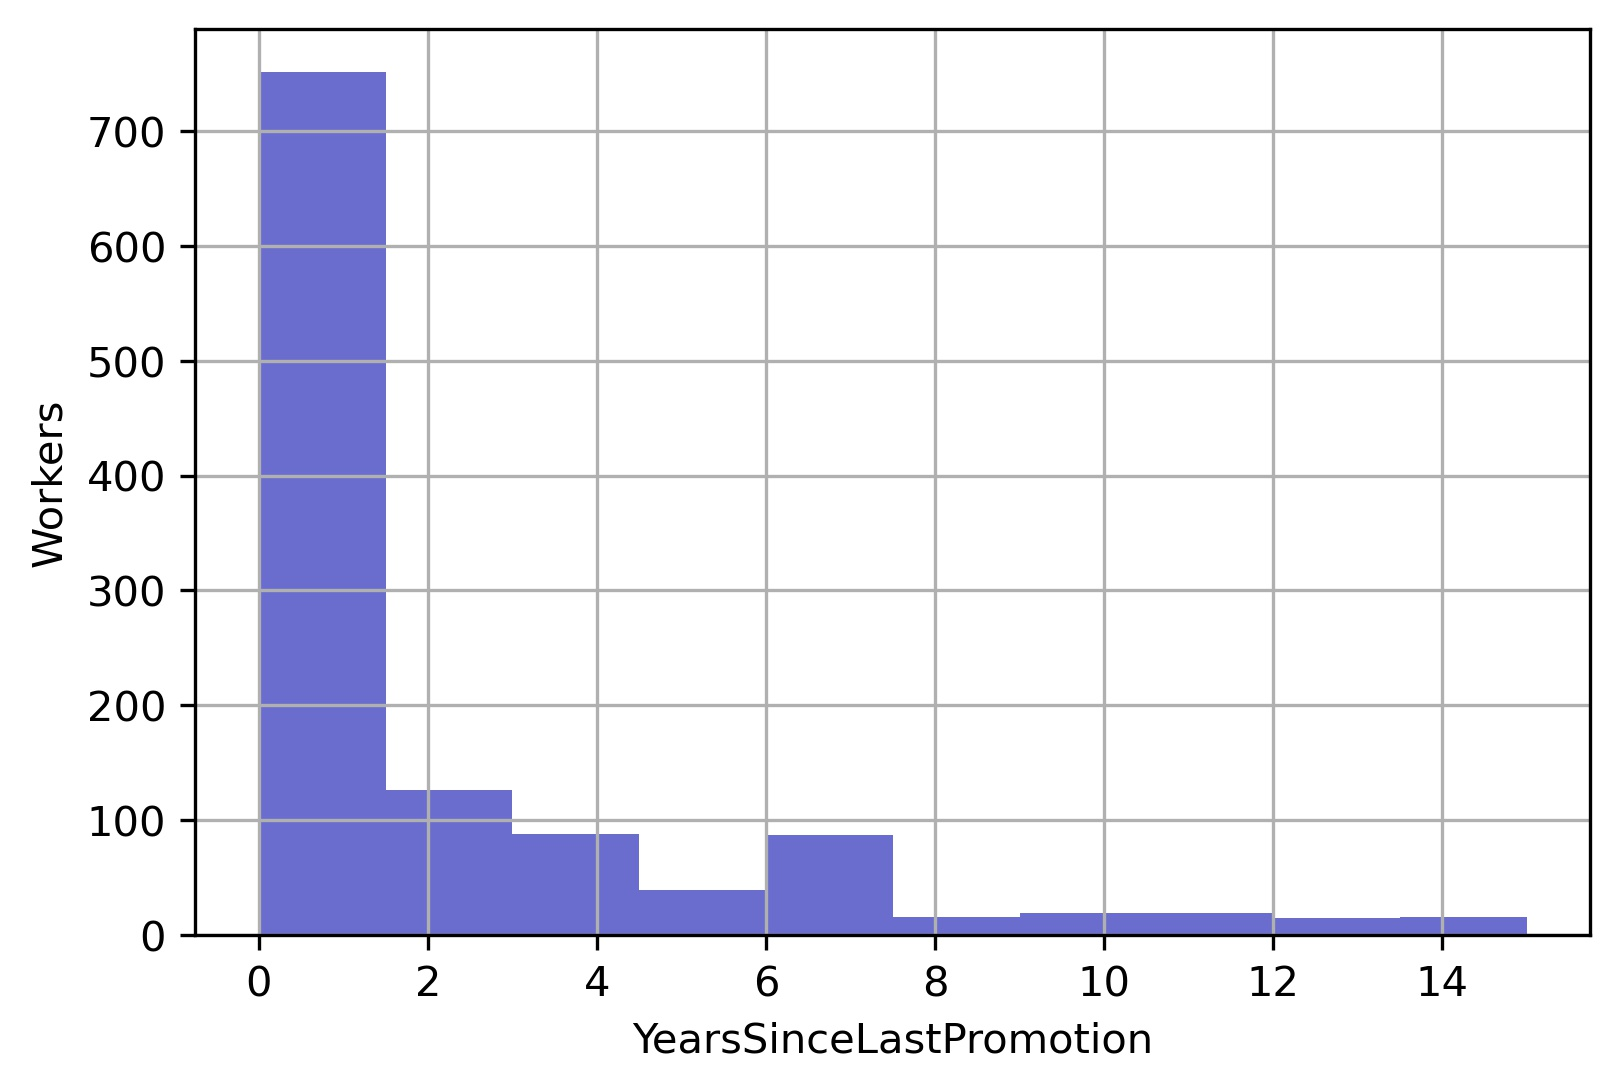
\includegraphics[width=.45\textwidth]{Immagini/YearsSinceLastPromotion.jpeg}
	}
	\quad
	\subfloat[]
	{
		\label{AttritionPromozione}
		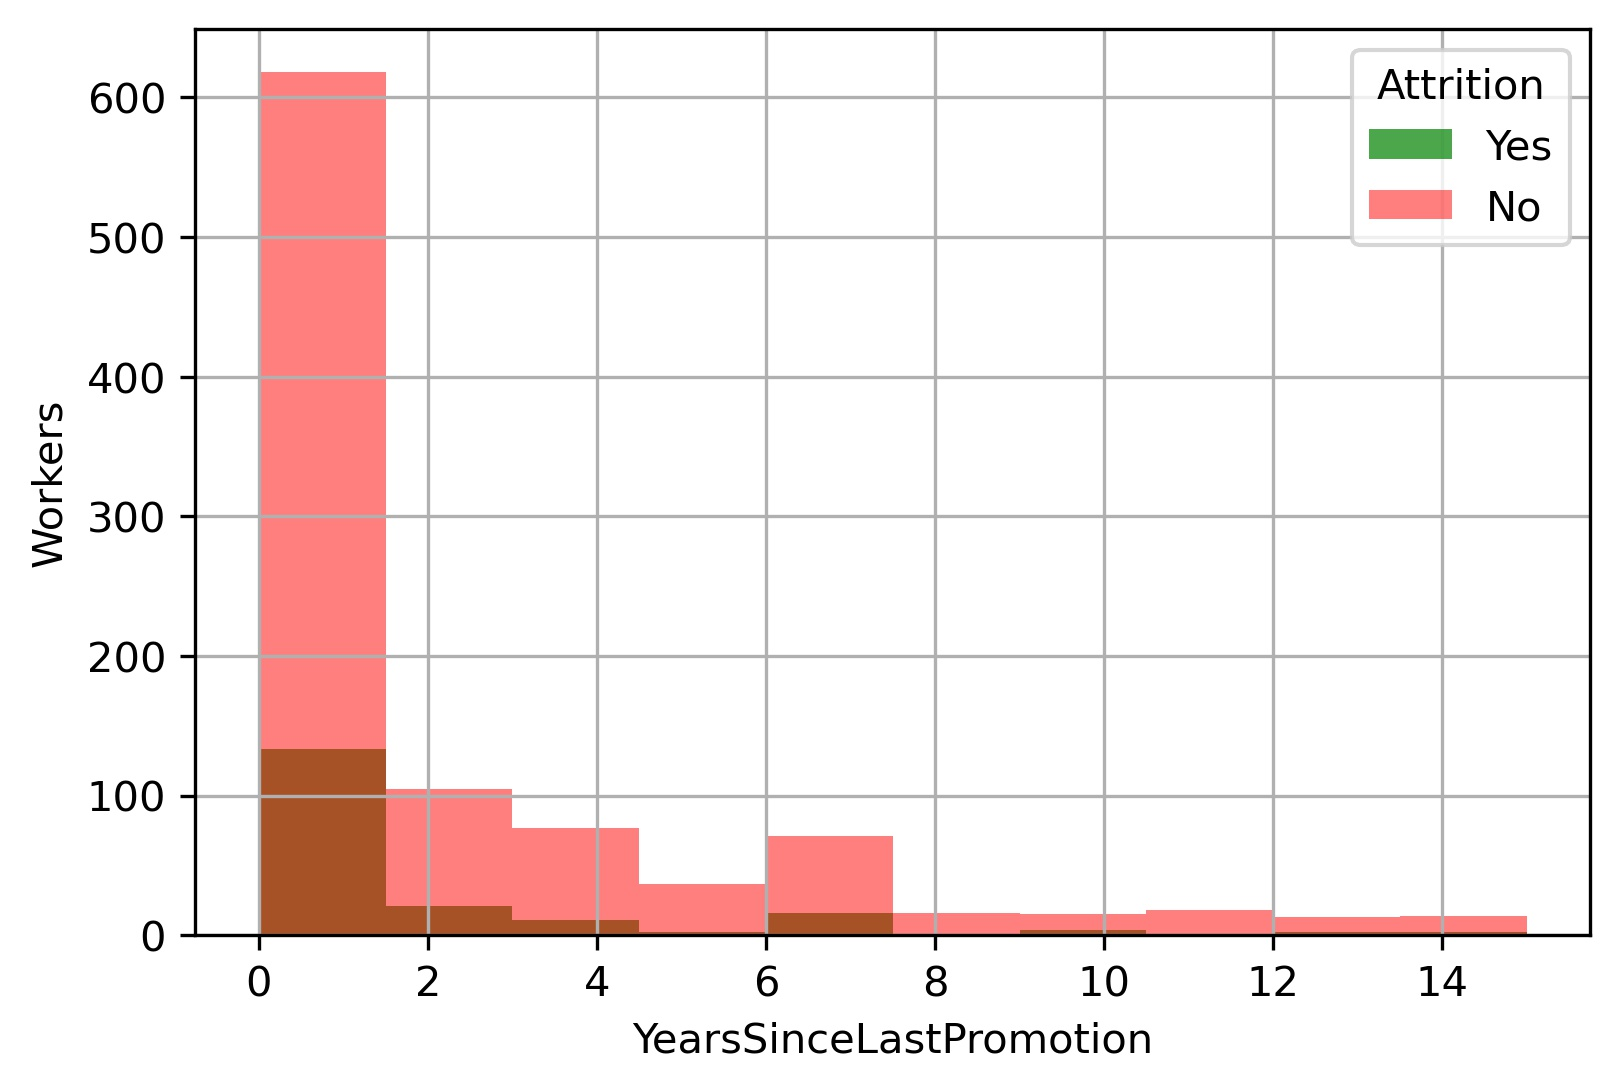
\includegraphics[width=.45\textwidth]{Immagini/Attrition_by_YearsSinceLastPromotion1.jpeg}
	}    \setlength{\belowcaptionskip}{-10pt}

	\caption{Distribuzione statistica degli anni dall'ultima promozione e del tasso di \textit{Attrition} in base allo stipendio}
	\label{GraficiPromozioneLavoro}
\end{figure}

\vspace{2em}

\begin{wrapfigure}{R}{0.50\textwidth}
    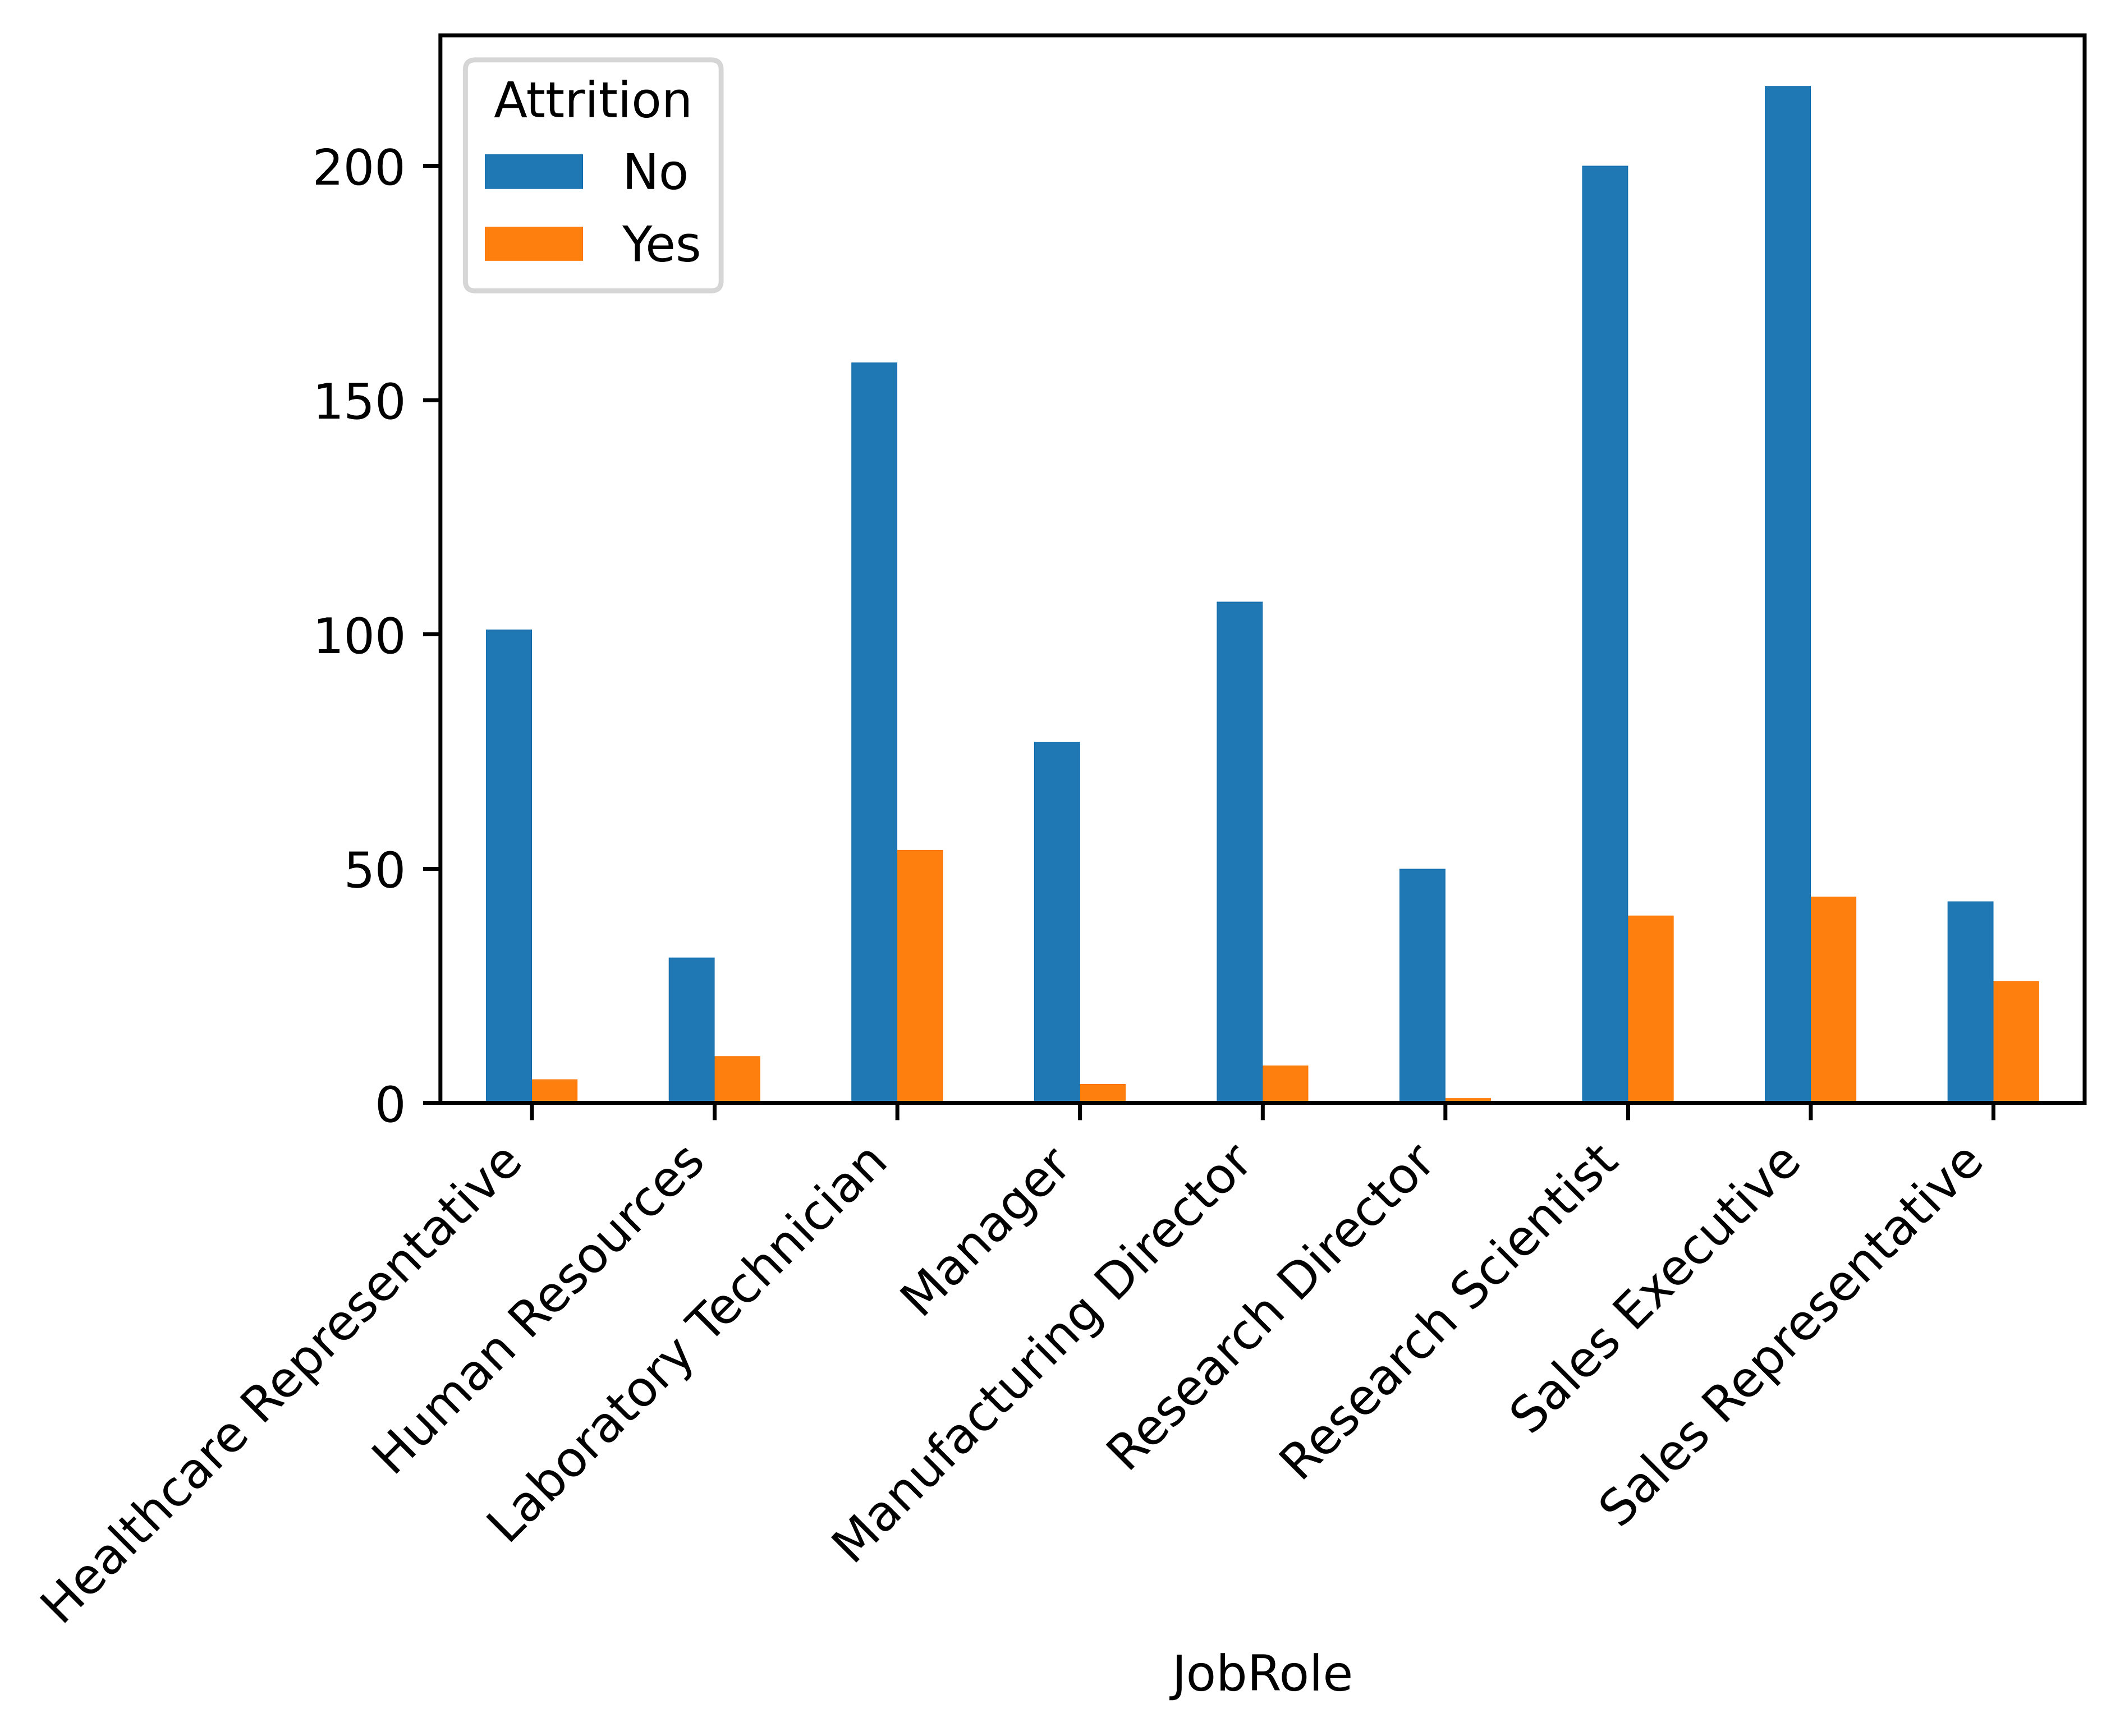
\includegraphics[width=0.49\textwidth]{Immagini/attritionRuolo.png}
    \setlength{\belowcaptionskip}{-10pt}
    \caption{Distribuzione della \textit{\textit{feature} Attrition} correlata al \textit{JobRole}}
     \clearpage
    \label{attritionJobRole}
\end{wrapfigure}

\noindent\textbf{\textit{JobRole}} è la posizione lavorativa di ciascun dipendente. Come viene evidenziato nella Figura \ref{attritionJobRole}, i lavoratori che tendono maggiormente a lasciare l'azienda sono \textit{Laboratory Technicians}, seguiti dai \textit{Research Scientists} e \textit{Sales Executives}. 
Vi sono, invece, pochissimi dipendenti che lasciano le posizioni di \textit{Manager} e \textit{Healthcare Representative} e addirittura nessuno che lascia la posizione di \textit{Research Director}.
%----ATTRITION GENDER
\\\\\textbf{\textit{Gender}} è l'attributo riguardante il sesso dei dipendenti. Dal grafico in Figura \ref{Attrition_Gender} notiamo che la quantità di persone che decidono di lasciare l'azienda è più equilibrata rispetto a quella osservata in \textit{JobRole}, sebbene in proporzione siano più gli uomini a prendere questa decisione rispetto alle donne. Abbiamo inoltre deciso di visualizzare la distribuzione del \textit{Gender} in base alla posizione lavorativa: anche in questo ambito le professioni appaiono più equamente distribuite tra i sessi (cfr. Figura \ref{JobRole_Gender}). Per le donne spiccano i valori associati a \textit{Laboratory Technician} e a \textit{Research Scientists}: in proporzione, infatti, risulta una maggior presenza di donne in questi settori rispetto agli uomini. Per i dipendenti di sesso maschile, invece, saltano all'occhio le professioni di \textit{Sales Executive} e \textit{Healthcare Representative}. \begin{figure}[H]
	\centering
	\subfloat[]
	{
		\label{Attrition_Gender}
		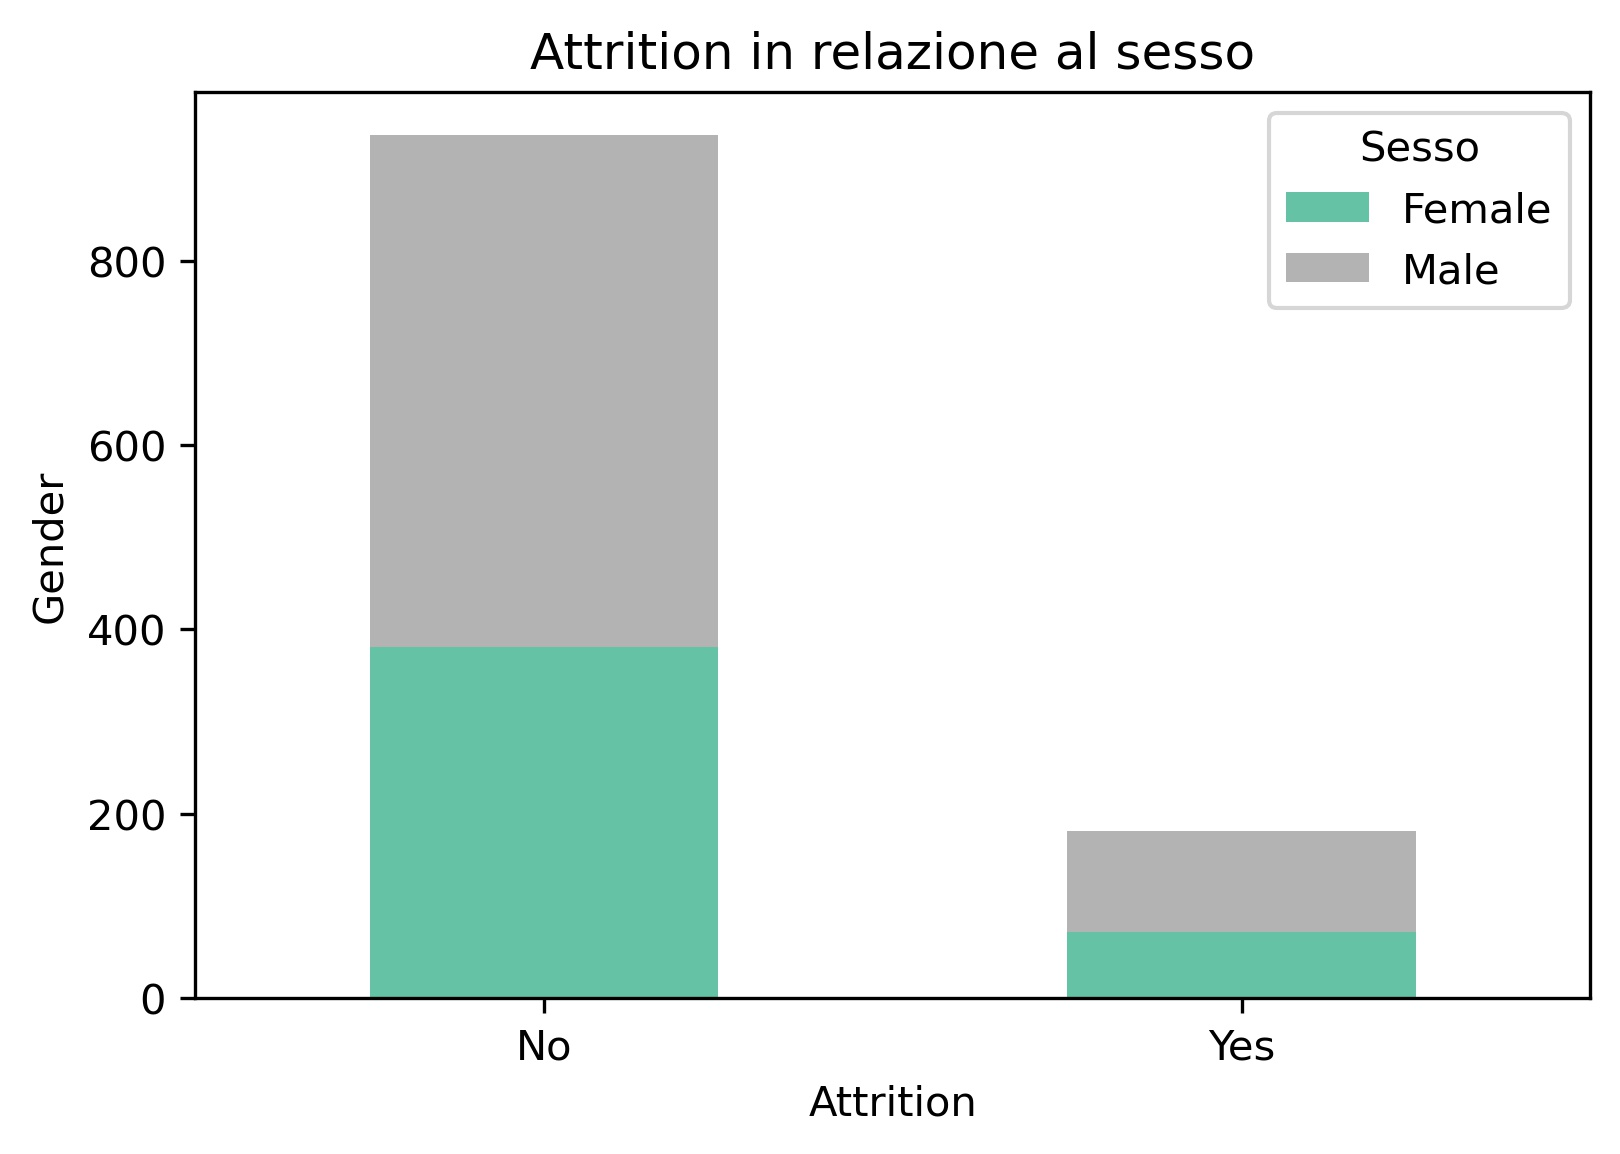
\includegraphics[width=.43\textwidth]{Immagini/Attrition_By_Gender1.jpeg}
	}
	\quad
	\subfloat[]
	{
		\label{JobRole_Gender}
		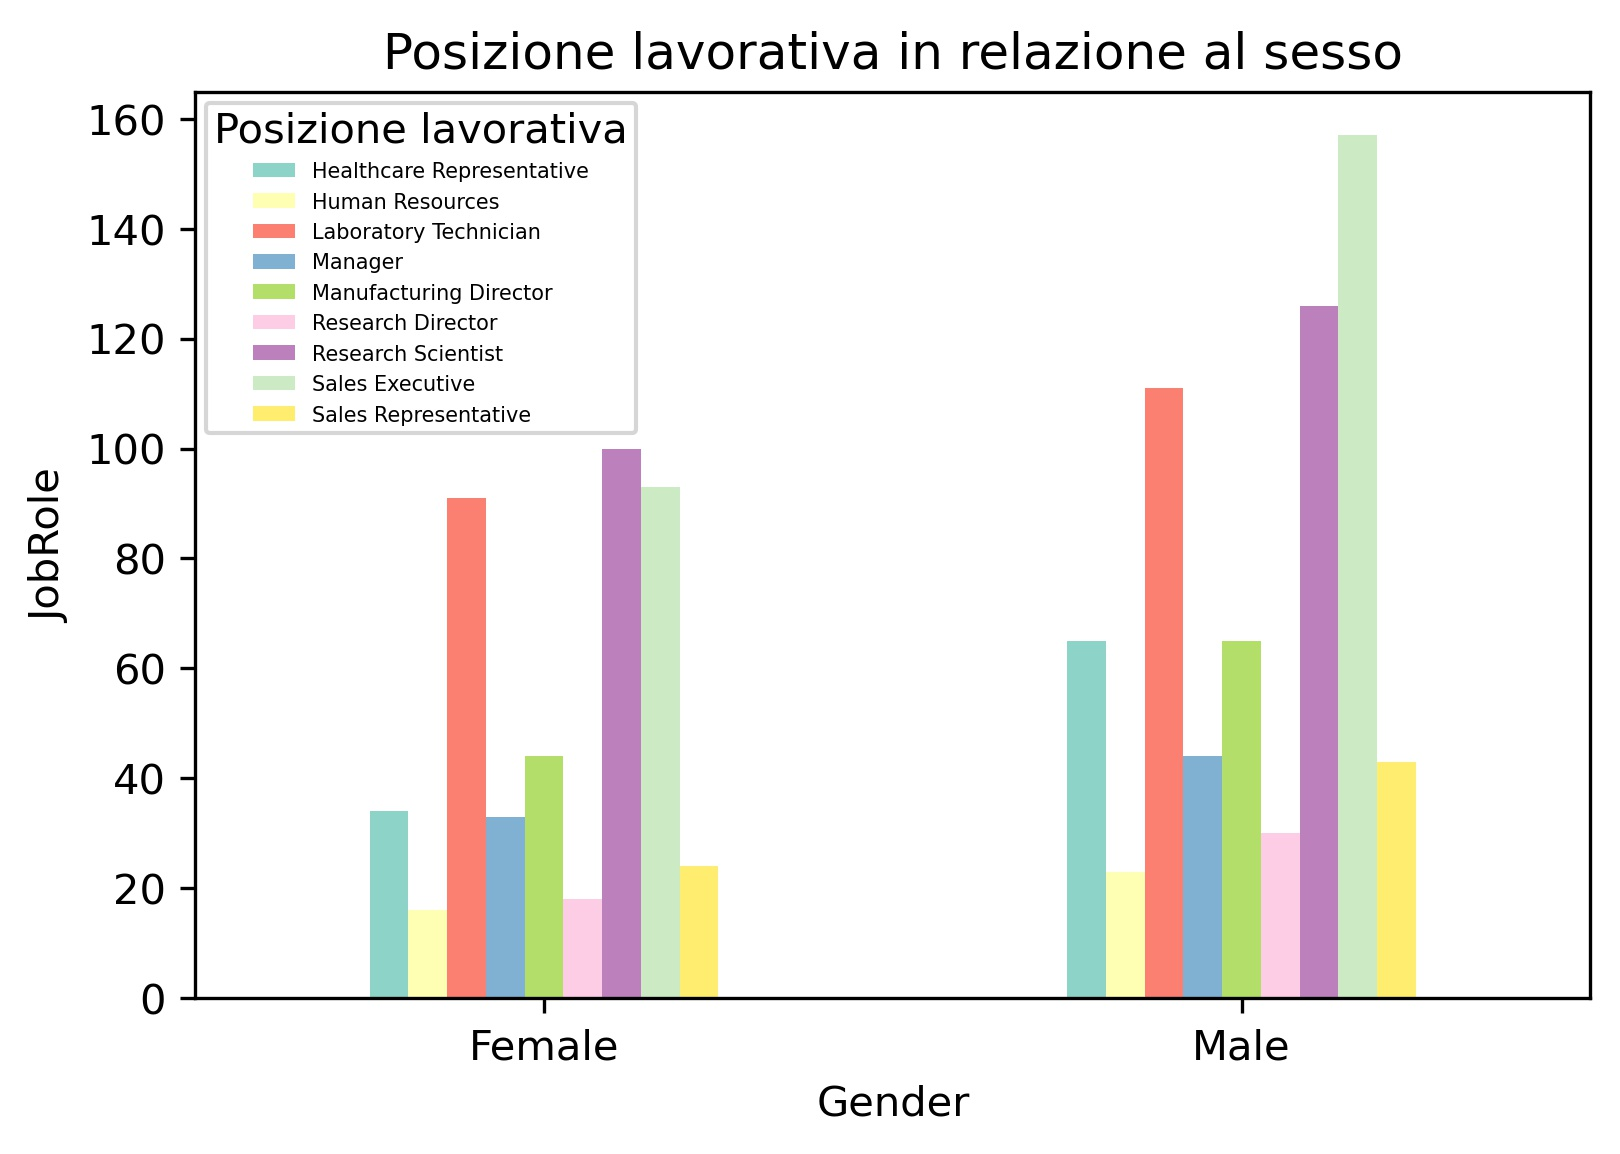
\includegraphics[width=.43\textwidth]{Immagini/JobRole_By_Gender1.jpeg}
	}
	\caption{Distribuzione dell'\textit{Attrition} in relazione al sesso dei lavoratori e distribuzione dei diversi ruoli svolti in base all'attributo \textit{Gender}}
	\label{GraficiAttrigionGenderJobRoleGender}
\end{figure}
\noindent Nella seguente tabella (Tabella \ref{statAttrNum}) abbiamo riportato le analisi statistiche applicate ai vari attributi numerici del dataset. Da questa si possono evincere alcuni valori chiave per lo studio dei dati, come ad esempio, l'età media dei lavoratori (37 anni circa) e lo stipendio mensile medio, minimo e massimo (in ordine 6566\$, 1009\$ e 19999\$). \\\\Inoltre, tenendo in considerazione le medie delle \textit{\textit{feature}} relative a \textit{Environment Satisfaction}, \textit{Job Satisfaction} e \textit{Relationship Satisfaction}, si nota che i dipendenti IBM sono  soddisfatti sia del proprio lavoro che dell'ambiente lavorativo aziendale. Infine, il livello medio di \textit{Education} tende a 3: tendenzialmente i lavoratori posseggono una laurea triennale (\textit{Bachelor's degree}).
\begin{table}[H]
\small
\centering
\resizebox{0.99\textwidth}{!}{
\begin{tabular}{|l|c|c|c|c|c|c|c|c|}
\hline
    \textbf{\textit{features}}            & \textbf{count}  & \textbf{mean}         & \textbf{std}         & \textbf{min}    & \textbf{25\%}    & \textbf{50\%}    & \textbf{75\%}     & \textbf{max}     \\ \hline\hline
Age                      & 1000.0 & 37.199000    & 9.015802    & 18.0   & 30.00   & 36.0    & 43.00    & 60.0    \\ \hline
DailyRate                & 1176.0 & 803.650510   & 406.683045  & 102.0  & 460.50  & 804.0   & 1169.00  & 1499.0  \\ \hline
DistanceFromHome         & 1176.0 & 9.210034     & 8.097024    & 1.0    & 2.00    & 7.0     & 14.00    & 29.0    \\ \hline
Education                & 1176.0 & 2.884354     & 1.016574    & 1.0    & 2.00    & 3.0     & 4.00     & 5.0     \\ \hline
EnvironmentSatisfaction  & 1176.0 & 2.715986     & 1.088876    & 1.0    & 2.00    & 3.0     & 4.00     & 4.0     \\ \hline
HourlyRate               & 1176.0 & 66.299320    & 20.266116   & 30.0   & 49.00   & 66.0    & 84.00    & 100.0   \\ \hline
JobInvolvement           & 1176.0 & 2.735544     & 0.716228    & 1.0    & 2.00    & 3.0     & 3.00     & 4.0     \\ \hline
JobLevel                 & 1176.0 & 2.021259     & 1.069686    & 1.0    & 1.00    & 2.0     & 3.00     & 5.0     \\ \hline
JobSatisfaction          & 1176.0 & 2.702381     & 1.101578    & 1.0    & 2.00    & 3.0     & 4.00     & 4.0     \\ \hline
MonthlyIncome            & 963.0  & 6565.946002  & 4710.625603 & 1009.0 & 2969.00 & 4969.0  & 8585.00  & 19999.0 \\ \hline
MonthlyRate              & 1176.0 & 14395.836735 & 7111.845106 & 2097.0 & 8227.25 & 14434.0 & 20489.25 & 26999.0 \\ \hline
NumCompaniesWorked       & 1176.0 & 2.663265     & 2.491287    & 0.0    & 1.00    & 2.0     & 4.00     & 9.0     \\ \hline
PercentSalaryHike        & 1176.0 & 15.176871    & 3.623941    & 11.0   & 12.00   & 14.0    & 18.00    & 25.0    \\ \hline
PerformanceRating        & 1038.0 & 3.152216     & 0.359403    & 3.0    & 3.00    & 3.0     & 3.00     & 4.0     \\ \hline
RelationshipSatisfaction & 1176.0 & 2.702381     & 1.092268    & 1.0    & 2.00    & 3.0     & 4.00     & 4.0     \\ \hline
StandardHours            & 606.0  & 80.000000    & 0.000000    & 80.0   & 80.00   & 80.0    & 80.00    & 80.0    \\ \hline
StockOptionLevel         & 1176.0 & 0.783163     & 0.851385    & 0.0    & 0.00    & 1.0     & 1.00     & 3.0     \\ \hline
TotalWorkingYears        & 1176.0 & 11.019558    & 7.694848    & 0.0    & 6.00    & 10.0    & 15.00    & 40.0    \\ \hline
TrainingTimesLastYear    & 943.0  & 2.827147     & 1.273120    & 0.0    & 2.00    & 3.0     & 3.00     & 6.0     \\ \hline
WorkLifeBalance          & 1176.0 & 2.755952     & 0.707984    & 1.0    & 2.00    & 3.0     & 3.00     & 4.0     \\ \hline
YearsAtCompany           & 1116.0 & 6.926523     & 6.063193    & 0.0    & 3.00    & 5.0     & 9.00     & 40.0    \\ \hline
YearsInCurrentRole       & 1176.0 & 4.188776     & 3.637405    & 0.0    & 2.00    & 3.0     & 7.00     & 18.0    \\ \hline
YearsSinceLastPromotion  & 1176.0 & 2.171769     & 3.189785    & 0.0    & 0.00    & 1.0     & 3.00     & 15.0    \\ \hline
YearsWithCurrManager     & 1176.0 & 4.107993     & 3.601097    & 0.0    & 2.00    & 3.0     & 7.00     & 17.0    \\ \hline
\end{tabular}
}    

\caption{\textit{Statistiche degli attributi numerici con totale dei valori, media, deviazione standard, valore minimo e massimo, quartili (25\%, 50\%, 75\%).}}
 \label{statAttrNum}
\end{table}
\noindent 
Passando all'analisi dei risultati in tabella \ref{StatAttrCat}, è possibile definire una migliore profilazione dei dipendenti IBM: sono prevalentemente di sesso maschile (il 56,46\% sul totale dei dipendenti), sposati, che hanno svolto studi legati alle scienze naturali o alle discipline sanitarie. All'interno dell'azienda, i dipendenti lavoravano prevalentemente come \textit{Sales Executive}, ricercatori o tecnici di laboratorio. Si può infine evidenziare come l'81,29\% non svolga viaggi di lavoro o li effettui raramente.
\begin{table}[H]
\small
\centering
\resizebox{0.99\textwidth}{!}{
\begin{tabular}{|p{3cm}|P{1.7cm}|P{2cm}|P{2.5cm}|P{2.7cm}|P{2.5cm}|}
\hline
\textbf{\textit{features}}&\textbf{Righe non vuote}& \textbf{Valori unici}& \textbf{1° valore più frequente (moda) }& \textbf{2° valore più frequente.}& \textbf{3° valore più frequente}\\
\hline
Attrition & 1176 & 2 & No (984) & Yes (192) & / \\ 
\hline
BusinessTravel & 1069 & 3 & Travel\_Rarely (764) & Travel\_Frequently (192) & Non-Travel (113)\\
\hline
Department & 1176 & 3& Research \& Development (769) & Sales (361) & Human Resources (46)\\
\hline
EducationField & 1176 & 6 & Life Sciences (489) & Medical (370) & Marketing (125) \\
\hline
Gender & 1117 &2 & Male (664) & Female (453) & / \\
\hline
JobRole & 1176 & 9 & Sales Executive (261) & Research Scientist (240) & Laboratory Technician (212) \\
\hline
MaritalStatus & 1176 & 3 & Married (542) &  Single (383) & Divorced (251) \\
\hline
Over18 & 804 & 1 & Y (804) & / & / \\
\hline
OverTime & 1176 & 2 & No (838) & Yes (338) & / \\
\hline
\end{tabular}
}
\caption{\textit{Descrizione statistica degli attributi categorici nominali con frequenza dei primi tre valori più ricorrenti.}}
\label{StatAttrCat}
\end{table}
\section{Valutazione della qualità dei dati}
\subsection{Valori mancanti}
Sono stati rilevati valori mancanti per gli attributi: \textit{Age}, \textit{BusinessTravel}, \textit{Gender}, \textit{Over18}, \textit{MonthlyIncome}, \textit{PerformanceRating}, \textit{StandardHours}, \textit{TrainingTimesLastYear} e \textit{YearsAtCompany}. \\\\
Non si è proceduto alla correzione di \textit{Over18}, \textit{StandardHours} e \textit{PerformanceRating}: i valori presenti non permettono di effettuare una stima soddisfacente delle controparti mancanti (cfr. \textit{Attributi problematici} nella Tab. \ref{TabAttributiProblematici} e, più sotto, le considerazioni su \textit{PerformanceRating}).\\\\I valori mancati di \textit{Age} e \textit{TrainingTimesLastYear} sono stati sostituiti con la media arrotondata all’intero più vicino, mentre nel caso di \textit{BusinessTravel} e \textit{Gender} con la moda. In tutti e quattro i casi, i valori sono stati calcolati tenendo come riferimento il rispettivo \textit{JobRole}, nel tentativo di offrire una stima quanto più accurata possibile. La media delle età dei lavoratori \textit{Sales Executive}, ad esempio, è 38 anni, mentre dei \textit{Research Director} 40.

\begin{table}[H]
\centering
\begin{tabular}{|l|c|l|P{3cm}|}
\hline
\multicolumn{2}{|c|}{Attributi corretti}                                           & \multicolumn{2}{c|}{Attributi problematici}                                                                                                                                                                                                         \\ \hline
\textbf{\textit{feature}} & \textbf{Valori mancanti} (\%) & \textbf{\textit{feature}}           & \textbf{Valori} \\ 
\hline
\textbf{Age} & 176 (15\%)   & \textbf{Over18}  & \textit{NaN} 372 (32\%) 
\newline \textit{Y} 804 (68\%)                                                                    \\ 
\hline
\textbf{Gender}  & 59 (5\%)                                       & \textbf{StandardHours}     & \textit{NaN} 570 (48\%)\newline \textit{80.0} 606 (52\%)                                                                                                                                    \\ \hline
\textbf{BusinessTravel}          & 107 (9\%)                                      & \textbf{PerformanceRating} & \begin{tabular}[c]{@{}l@{}}\textit{NaN} 138 (18\%)\\ \newline\textit{3.0} 808 (69\%)\\ \newline \textit{4.0} 158 (13\%)\end{tabular} \\ \hline
\end{tabular}
\caption{Valori mancanti: attributi corretti e problematici}
    \label{TabAttributiProblematici}
    \end{table}
    
\subsection{Errori nel dataset}
In \textit{MonthlyIncome} e \textit{YearsAtCompany} ai valori mancanti si accompagnano svariati errori di correttezza semantica.\\\\
Il confronto fra \textit{YearsAtCompany} e gli analoghi attributi \textit{TotalWorkingYears}, \textit{YearsInCurrentRole}, \textit{YearsSinceLastPromotion} e \textit{YearsWithCurrManager}, o con \textit{Age} e \textit{NumCompaniesWorked}, mostra in molti casi valori contraddittori\footnote{Ad esempio, \textit{TotalWorkingYears} dovrebbe essere sempre superiore a \textit{YearsAtCompany} e, trattandosi IBM di una compagnia statunitense, la differenza fra qualsiasi parametro riferito agli anni lavorativi e \textit{Age} non dovrebbe mai essere superiore a 14.}. \\\\ Singolarmente, \textit{YearsAtCompany} non mostra poi alcuna correlazione con \textit{Attrition}. Si è notato che rimuovendo gli \textit{outlier} si ha un lieve aumento della correlazione, che rimane tuttavia al di sotto di quella degli altri attributi. Si è quindi scelto di mantenere come solo parametro riferito agli anni \textit{YearsInCurrentRole}. Per i fini del presente \textit{paper} è infatti il più interessante, mostrando una discreta correlazione con \textit{Attrition}, e la quasi perfetta corrispondenza fra suoi i valori e quelli presenti in \textit{YearsWithCurrManager} rende plausibile supporne una buona correttezza.\\\\
Analogamente si è proceduto con \textit{MonthlyIncome}, \textit{HourlyRate},  \textit{DailyRate} e \textit{MonthlyRate}, tutti quanti contraddittori fra loro. Rimuovendo gli outlier e sostituendo i valori mancanti (con la metodologia di cui sopra), \textit{MonthlyIncome} ha mostrato una correlazione con \textit{Attrition} ed è stato l'unico attributo mantenuto. 

\subsection{Rimozione degli \textit{outlier}}
Per l’analisi di alcuni degli attributi del paragrafo precedente si è fatto ricorso alla rimozione degli \textit{outlier}, individuati con l’uso di \textit{boxplot}. Di ciascun parametro è stato poi calcolato l’\textit{IQR} e si è proceduto alla rimozione dei valori non appartenenti al \textit{range interquartile}.\\\\
La stessa operazione è stata effettuata per \textit{YearsInCurrentRole}. I (pochi) \textit{outlier} rilevati confermano ulteriormente la validità di questo attributo. Nella Fig. \ref{boxplotOutliers} gli \textit{outlier} di \textit{YearsInCurrentRole} a confronto con quelli di \textit{YearsAtCompany}.
\vspace{2em}
\begin{figure}[H]
    \centering
    \small
    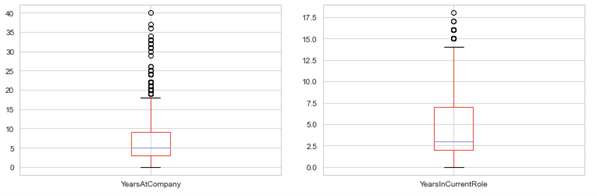
\includegraphics[width=0.68\textwidth]{Immagini/boxplot.png}
    \caption{Boxplot per \textit{YearsAtCompany} e \textit{YearsInCurrentRole}}
    \label{boxplotOutliers}
\end{figure}
\subsection{Creazione di attributi}
Per agevolare l’analisi del dataset, sono stati creati due nuovi attributi in luogo di altri già esistenti.
\begin{itemize}
\itemsep0em
    \item \textit{\textbf{GeneralEmployeeSatisfaction}}: include la media approssimata all’intero più vicino dei valori riguardanti la soddisfazione del dipendente: \textit{EnvironmentSatisfaction}, \textit{JobSatisfaction}, \textit{RelationshipSatisfaction};
    \item \textbf{\textit{CompanyInvolvement}}: include la media approssimata all’intero più vicino dei valori degli attributi indici del coinvolgimento del dipendente con le dinamiche aziendali: \textit{StockOptionLevel} e \textit{JobInvolvement}. Si noti che il primo parametro era in scala 0-3, il secondo 1-4: i valori di \textit{StockOptionLevel} sono stati dunque convertiti.
\end{itemize}

\subsection{Trasformazione dei valori}
I valori di alcuni attributi di tipo stringa sono stati convertiti in numerici\footnote{Per praticità, nel dataframe tali attributi sono stati siglati con * (es. \textit{Attrition*}).}. In particolare:
\begin{itemize}
\itemsep0em 
    \item \textit{\textbf{Attrition}}: NO $\rightarrow$ 0,  YES $\rightarrow$ 1;
    \item \textit{\textbf{Business Travel}}: Non\_Travel $\rightarrow$ 0,  Travel\_Rarely $\rightarrow$ 1,  Travel\_Frequently $\rightarrow$ 2.
    \item \textit{\textbf{Department}}: Human Resources $\rightarrow$ 0,  Research \& Development  $\rightarrow$ 1, Sales $\rightarrow$ 2;
    \item \textit{\textbf{EducationField}}: Human Resources $\rightarrow$ 0, Life Sciences $\rightarrow$ 1, Marketing $\rightarrow$ 2, Medical $\rightarrow$ 3, Other $\rightarrow$ 4, Technical Degree $\rightarrow$ 5;
    \item \textbf{\textit{Gender}}: Female $\rightarrow$ 0, Male $\rightarrow$ 1; 
    \item \textit{\textbf{JobRole}}: Healtcare Rappresentative $\rightarrow$ 0, Human Resources $\rightarrow$ 1, Laboratory Technician $\rightarrow$ 2, Manager $\rightarrow$ 3, Manufacturing Director $\rightarrow$ 4, Research Director $\rightarrow$ 5, Research Scientist $\rightarrow$ 6, Sales Executive $\rightarrow$ 7, Sales Rappresentative $\rightarrow$ 8;
    \item \textit{\textbf{MaritalStatus}}: Divorced $\rightarrow$ 0, Married $\rightarrow$ 1, Single $\rightarrow$ 2;
    \item \textbf{\textit{OverTime}}: No $\rightarrow$ 0, Yes $\rightarrow$ 1.
\end{itemize}

\subsection{Rimozione di \textit{\textit{feature}}}
La correzione degli errori e la conversione dei sopracitati valori (in particolare dell'attributo-chiave \textit{Attrition}) permettono di computare una prima \textit{matrice di correlazione}. Da essa, possiamo notare quali siano gli attributi più importanti e quali invece non abbiano alcuna particolare relazione con \textit{Attrition}. \\\\
Alla luce dei rilevamenti finora segnalati, dal dataset sono stati eliminati i seguiti attributi, oltre a quelli già citati:
\begin{itemize}
    \itemsep0em
    \item \textit{\textbf{StandardHours}} e \textbf{\textit{Over18}}: i valori non mancanti sono identici l’un l’altro, non offrendo alcuna informazione utile. \textit{Over18} risulta inoltre ridondante con \textit{Age};
    \item \textbf{\textit{PerformanceRating}}: rispetto ai due casi precedenti, i valori mancanti sono relativamente più contenuti e a livello intuitivo il parametro sarebbe stato potenzialmente molto utile per l’analisi di \textit{Attrition}. Tuttavia, l’ampia presenta di “3” a scapito di “1” e “2” (che non hanno alcuna occorrenza) inficia gravemente i possibili utilizzi di questo parametro e, a nostro avviso, la sua generale validità. È stato pertanto scartato;
    \item \textbf{\textit{Education}}, \textit{\textbf{BusinessTravel}}, \textit{\textbf{TrainingTimesLastYear}}, \textit{\textbf{NumCompaniesWorked}}, \textit{\textbf{PercentSalaryHike}}: scarsa o nulla correlazione con \textit{Attrition};
    \item \textit{\textbf{JobRole}}: il parametro è stato utile per correggere i dati mancanti, ma per le successive analisi risulta ridondante, con la presenza del più compatto \textit{Department};
    \item	\textbf{\textit{EducationField}}: nessuna correlazione con \textit{Attrition}. Per questo parametro abbiamo verificato se l’eventuale discrasia fra \textit{EducationField} e \textit{Department} possa essere una possibile causa di \textit{Attrition}, ottenendo risposta negativa. %(cfr. Figura \ref{fig:eduField}).
\end{itemize}
%\begin{figure}[H]
%    \centering
%    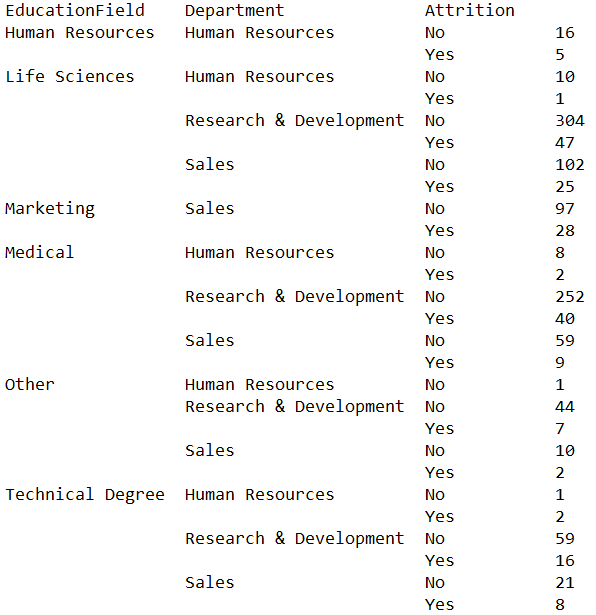
\includegraphics[scale = 0.7]{Immagini/edufield.jpg}
%    \caption{Confronto tra \textit{EducationField}, \textit{Department} e \textit{Attrition}}
%    \label{fig:eduField}
%\end{figure}
A seguito della nostra operazione di \textit{data cleaning} abbiamo ottenuto un dataset di 1029 oggetti descritti da 13 attributi. Di seguito la relativa matrice di correlazione (sono esclusi \textit{Department} e \textit{MaritalStatus}, parametri non binari originariamente categorici).
\vspace{2em}
\begin{figure}[H]
    \centering
    %\subfloat[]{{\includegraphics[scale=0.3]{Immagini/neomatrix.png} }}
    %\quad
    %\subfloat[]{{
    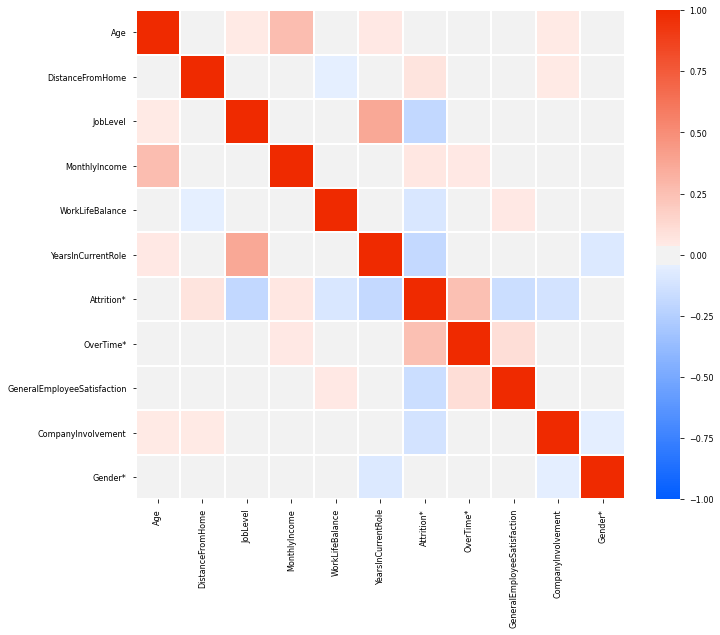
\includegraphics[scale=0.50]{Immagini/neoMatrix.png} %}}
    \caption{Matrice di correlazione dopo l'operazione di \textit{data cleaning}}
    \label{fig:MatrCorrelPostDataClean}
\end{figure}



    
    \section{Clustering}
A seguito del \textit{data cleaning} si è proceduto al clustering del dataset, utilizzando come attributi di riferimento quelli che maggiormente descrivono la situazione del lavoratore all’interno un’azienda e possono determinarne l’\textit{Attrition}: \textit{MonthlyIncome}, \textit{DistanceFromHome}, \textit{JobLevel} e \textit{OverTime}. Tutti e quattro i parametri hanno inoltre mostrato in una qualche misura correlazione con \textit{Attrition}, come visto nella matrice. Lo scopo dell’operazione è stato suddividere i dipendenti in cluster con attributi correlati l’un l’altro.
Sono stati utilizzati tre tipi di algoritmi di clustering: il \textit{K-Means}, il \textit{DBSCAN} e il \textit{Gerarchico} (nelle sue varie declinazioni). Prima dell’applicazione di ciascun algoritmo è stato necessario effettuare lo \textit{scaling} dei dati (attraverso il \textit{MinMaxScaler}). Successivamente, sono stati valutati i parametri ottimali e, infine, la bontà dei risultati ottenuti.
\subsection{\textit{K-Means}}
La corretta applicazione dell’algoritmo \textit{K-Means} è legata alla scelta del \textit{parametro K}, che rappresenta il numero di cluster in cui il dataset verrà suddiviso. Per rilevare il corretto valore di\textit{ K} abbiamo utilizzato il \textit{Knee Method}, dopo aver rappresentato graficamente il possibile \textit{SSE (Sum of Squared Errors)} per differenti quantità di cluster comprese fra 2 e 50. Dall’analisi della figura \ref{fig:SSE}, si è notato che l’ideale valore di \textit{K} è 4. Si è quindi calcolato il relativo \textit{coefficiente di Silhouette}, pari a 0.397. Con valori di \textit{K} più grandi si è notata una diminuzione del valore della \text{Silhouette}. Con \textit{K} pari a 3 l’aumenta del valore è minimo (0.407), mentre avere soltanto due cluster (\textit{Silhouette} = 0.518) sarebbe poco utile per i nostri scopi.
\begin{figure}[H]
    \centering
    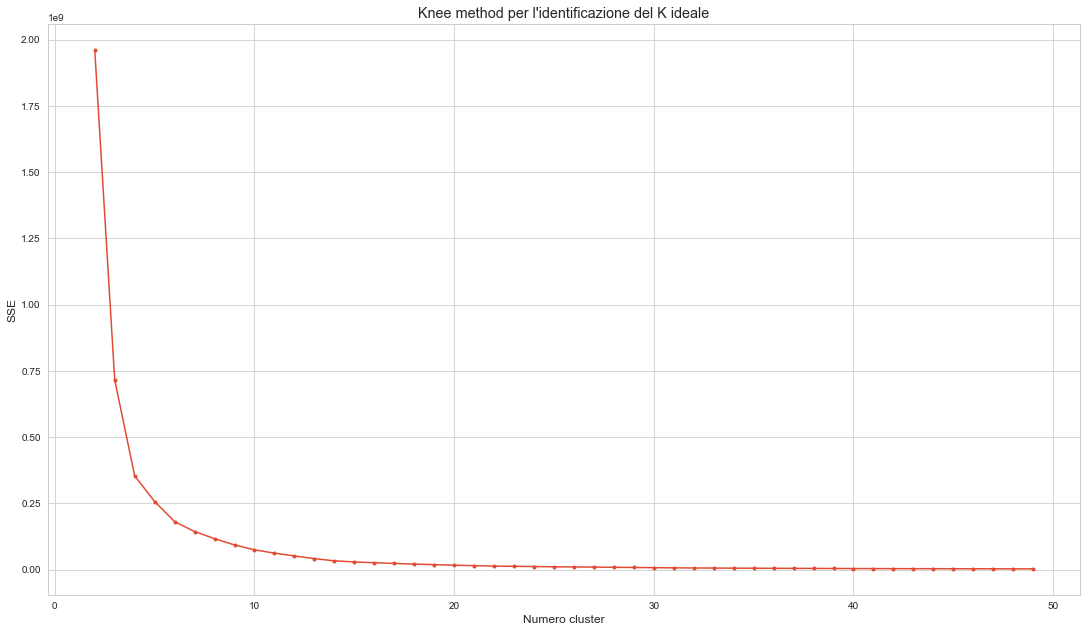
\includegraphics[scale=0.25]{Immagini/SSE.png}
    \caption{SSE con K da 2 a 50}
    \label{fig:SSE}
\end{figure}
\noindent Di seguito il grafico delle \textit{Parallel Coordinates} dei quattro cluster individuati e la tabella che quantifica la popolazione di ciascun cluster. Tutti i cluster sono accomunati da un simile valore medio per \textit{MonthlyIncome} e – a eccezione del Cluster 2 – assenza di \textit{OverTime}. Sempre il Cluster 2 spicca per il \textit{JobLevel} più alto della media. Valori più alti della media si rilevano anche nel Cluster 4 per la \textit{DistanceFromHome}, invece molto bassa per i lavoratori del Cluster 1. 
\begin{figure}[H]
\resizebox{.99\textwidth}{!}{
\centering
\hfill
\begin{minipage}{0.6\textwidth}
  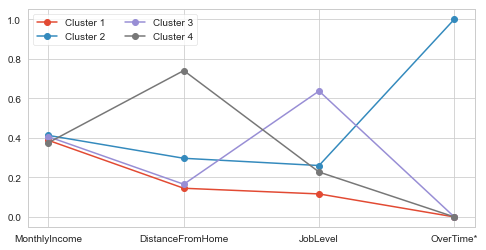
\includegraphics[scale = 0.5]{Immagini/parallelKmeans.png}
    \label{parallelCoord}
    \caption{\textit{Parallel Coordinates} dei \\ cluster}
\end{minipage}
\quad
\begin{minipage}{0.4\textwidth}
\centering
 \begin{tabular}{|c|P{3cm}|}
        \hline    
        \textbf{Cluster} & \textbf{Numero dipendenti nel cluster} \\
        \hline
        0 & 417 \\
        \hline
        1 & 301\\
        \hline
        2 & 137 \\
        \hline
        3 & 174 \\
        \hline
    \end{tabular}
  \captionof{table}{Distribuzione dei dipendenti nei cluster}
\end{minipage}\hspace*{\fill}}
\end{figure}
\noindent\\Si è poi passati a osservare la distribuzione dei vari parametri, a cominciare da \textit{Attrition}. Essa appare pressoché identica fra i Cluster 1 e 4, con una lieve diminuzione nel Cluster 3 e un significativo aumento nel Cluster 2 dovuto, probabilmente, alla presenza di \textit{OverTime} che abbiamo rilevato. I Cluster 2 e 4 contengono inoltre una relativa alta concentrazione di dipendenti con bassa \textit{WorkLifeBalance}.
\\\\
Una possibile spiegazione della bassa concentrazione di \textit{Attrition} nel Cluster 3 – già notato per l’alto \textit{JobLevel} - è data dalla distribuzione di \textit{YearsInCurrentRole}: oltre tre quinti dei dipendenti sono infatti in azienda da più di sei anni. Di contro, i dipendenti del Cluster 1, oltre ad avere un \textit{JobLevel} più basso, sono anche in azienda da meno tempo.
\\\\
I valori di \textit{WorkLifeBalance} e \textit{DistanceFromHome} del Cluster 4 non sembrano essere motivo di \textit{Attrition}, a discapito di quanto si potrebbe pensare intuitivamente (e quanto potrebbe emergere dalla matrice di correlazione). Essi sono forse mitigati dalla concentrazione sopra la media di dipendenti con alto livello di \textit{CompanyInvolvement}.
\\\\
Attributi non direttamente legati alla vita aziendale dell’impiegato, come \textit{MaritalStatus} o \textit{Gender}, risultano invece equamente distribuiti e non degni di nota.
\\\\
Complessivamente, il metodo \textit{K-Means} è riuscito ad analizzare il dataset in modo significativo, mettendo in evidenza alcuni attributi che possono influenzare (in positivo o in negativo) l’\textit{Attrition} dei vari dipendenti.
\begin{figure}[H]
	\centering
	\subfloat 
	{
		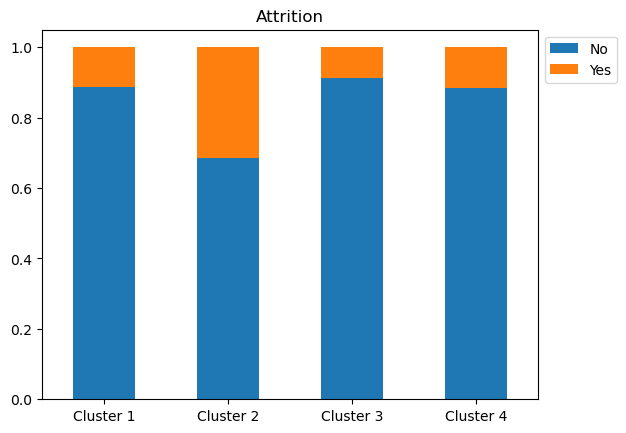
\includegraphics[width=.45\textwidth]{Immagini/KMeansAttr.png}
		\label{kmeansAttrition}
	}
	\quad
	\subfloat
	{
		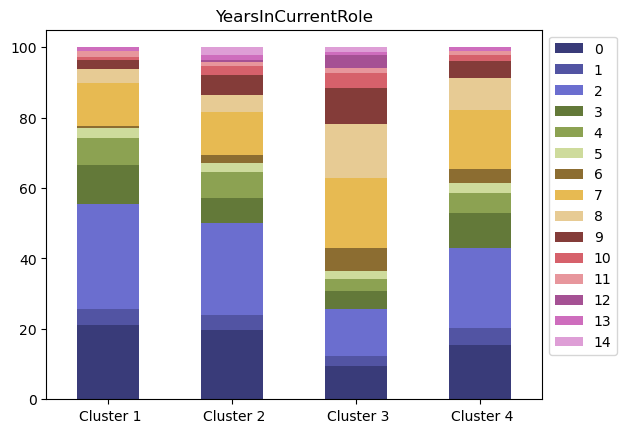
\includegraphics[width=.45\textwidth]{Immagini/KMeansYears.png}
		\label{kmeansYears}
    }
	\label{Cluster}
\end{figure}
\begin{figure}[htp]
\centering
		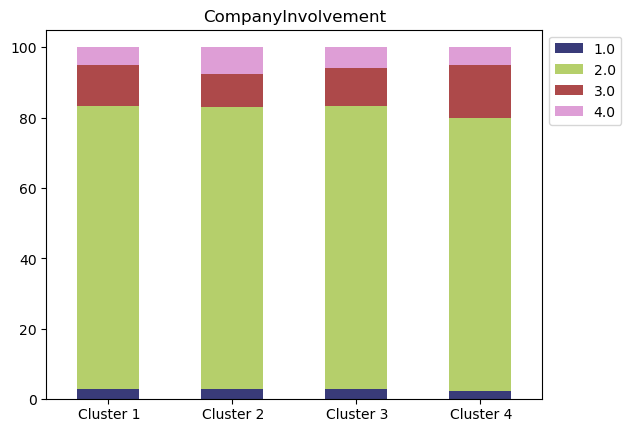
\includegraphics[width=.30\textwidth]{Immagini/KMeansCompanyInv.png}
		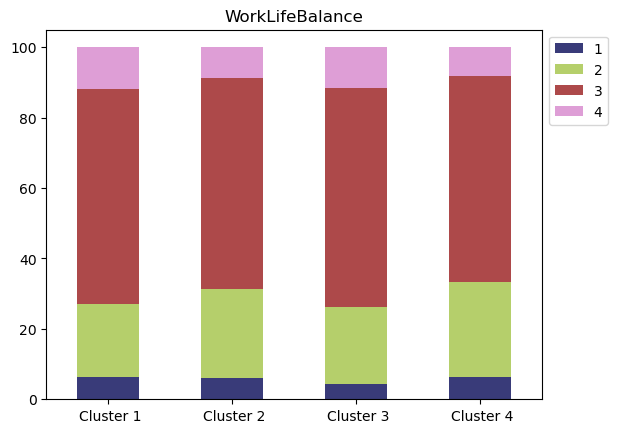
\includegraphics[width=.30\textwidth]{Immagini/KMeansWorkLife.png}
		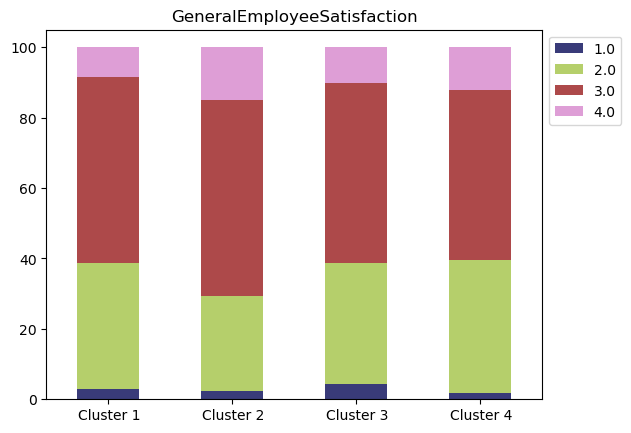
\includegraphics[width=.30\textwidth]{Immagini/KMeansGeneralEmp.png}
		\caption{Distribuzione degli attributi \textit{Attrition}, \textit{YearsInCurrentRole}, \textit{CompanyInvolvement}, \textit{WorkLifeBalance}.\textit{GeneralEmployeeSatisfaction} all'interno dei quattro cluster ottenuti}
\end{figure}
\subsection{\textit{DBSCAN}}
Il metodo di clustering \textit{DBSCAN} si è dimostrato inefficace per il nostro dataset, fortemente sbilanciato con un’alta concentrazione di valori con \textit{Attrition} negativa. L’assunto iniziale – che l'\textit{Attrition} sia determinata da un insieme di più attributi correlati l’un l’altro – sottintende poi un insieme di dati a più dimensioni. Le varie relazioni che intercorrono fra i vari parametri, di cui si è accennato sopra analizzando i risultati del \textit{K-Means}, non possono essere correttamente visualizzate dal \textit{DBSCAN}, che opera in due dimensioni.
\begin{figure}
    \centering
  %  \vspace{-10mm}
    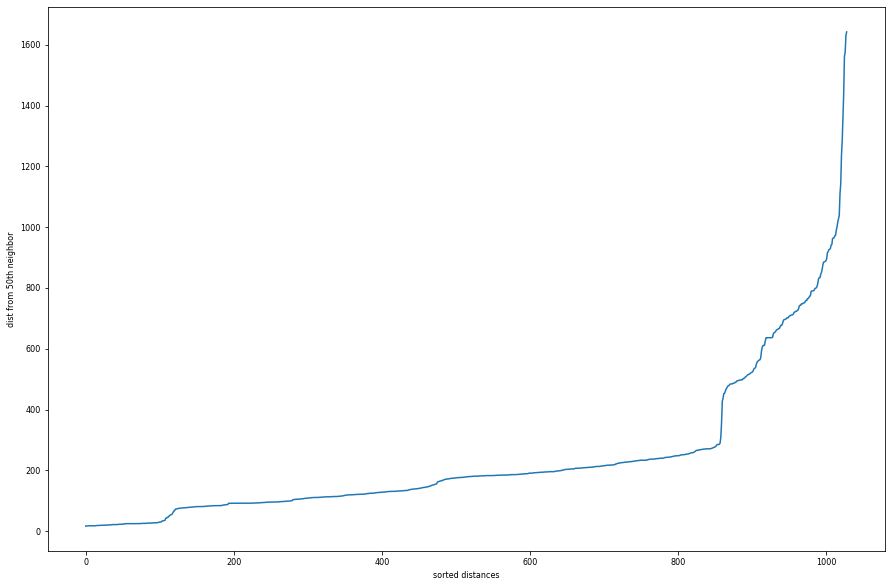
\includegraphics[scale = 0.25]{Immagini/dbscanKnee.png}
    \caption{Grafico \textit{Knee-method}}
    \label{fig:KneeDBSCAN}
    \captionsetup{belowskip=0pt}
\end{figure}                                                                                                                                                                                                                                                                    
\noindent Dopo aver determinato 0.25 come valore ottimale di \textit{EPS} (cioè il raggio dell'intorno di ciascun punto) ricorrendo al \textit{Knee Method} (Fig.\ref{fig:KneeDBSCAN}), si è verificato che l’algoritmo genera il modello con il migliore valore di \text{Silhouette} (0.26) fissando \textit{minPts} (ovvero il numero minimo di punti che un punto deve avere nel suo intorno per essere definito \textit{core}) pari a 4.
\begin{figure}[H]
\resizebox{.99\textwidth}{!}{
\centering
\hfill
\begin{minipage}{0.6\textwidth}
  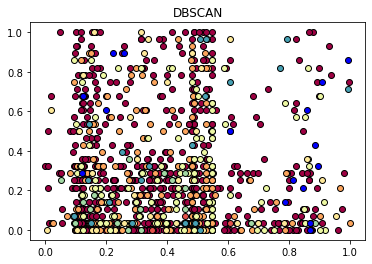
\includegraphics[scale = 0.65]{Immagini/DBSCAN.png}
    
    \caption{\textit{DBSCAN}
    \label{dbScan}}
\end{minipage}
\quad
\begin{minipage}{0.4\textwidth}
\vspace{1em}
\centering
 \begin{tabular}{|c|P{3cm}|}
        \hline    
        \textbf{Cluster} & \textbf{Numero dipendenti} \\
        \hline
        Cluster 1 & 663 \\
        \hline
        Cluster 2 & 7\\
        \hline
        Cluster 3 & 143 \\
        \hline
        Cluster 4 & 44 \\
        \hline
        Cluster 5 & 116\\
        \hline
        Cluster 6 & 19\\
        \hline
        Cluster 7 & 21\\
        \hline
        Rumore & 16 \\
        \hline
        \end{tabular}
  \captionof{table}{Distribuzione dei dipendenti nei cluster}
\end{minipage}\hspace*{\fill}}
\end{figure}
\noindent
Nello spazio sono tuttavia visualizzati dei punti senza alcuna apparente relazione fra loro (Fig. \ref{dbScan}), divisi in otto diversi cluster, di cui uno riservato al rumore. Tali cluster sono molto più sbilanciati di quelli analizzati con il \textit{K-Means}: abbiamo infatti un cluster eccessivamente grande, due medi e gli altri molto piccoli. Analoghi risultati sono stati ottenuti con altri valori di \textit{minPts}.
\\\\
Il basso valore della \textit{Silhouette}, i limiti intrinseci al metodo e lo sbilanciamento dei risultati forniti dal modello fanno propendere contro l’utilizzo del \textit{DBSCAN}.

\subsection{Clustering gerarchico}
Il terzo criterio di clustering sperimentato è quello gerarchico, che a sua volta ammette più possibili applicazioni: sono stati testati alberi gerarchici generati con l’algoritmo \textit{Single Link} (o \textit{MIN}), \textit{Complete} (o \textit{MAX}) e \textit{Average}. In tutti i casi è stato necessario impostare un diverso \textit{threshold} per ottenere un certo numero di cluster. Nel nostro caso, dovendo confrontare i risultati del metodo gerarchico con quelli ottenuti mediante \textit{K-Means}, abbiamo cercato di ottenere sempre quattro cluster.

\begin{table}[H]
\centering
\begin{tabular}{|l|c|c|S|}
\hline
\multicolumn{1}{|c|}{\textbf{Metodo}} & \multicolumn{1}{c|}{\begin{tabular}[c]{@{}c@{}}\textbf{Grandezza} \\ \textbf{cluster}\end{tabular}} & \multicolumn{1}{c|}{\textbf{Threshold}} & \multicolumn{1}{c|}{\textbf{Silhouette}} \\ \hline
Complete   & 69, 232, 180, 548   & 1.4  &   0.33777407417668387          \\ \hline
Average           & 726, 293, 8, 2   & 0.85    &    0.3784611202348606    \\ \hline
Single           & 728, 298, 2, 1   & 0.28 &  0.44019713225483575   \\  \hline
\end{tabular}
\caption{Differenti parametri impostati per il clustering gerarchico}
\end{table}

\begin{figure}[H]
\centering
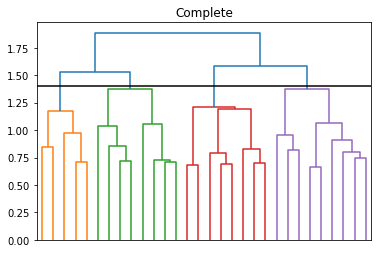
\includegraphics[width=.3\textwidth]{Immagini/GeraComplete.png}\hfill
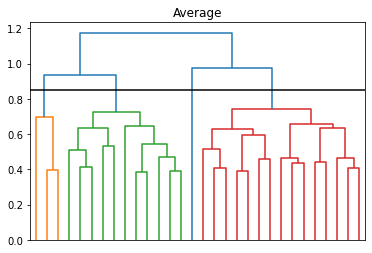
\includegraphics[width=.3\textwidth]{Immagini/GeraAvg.png}\hfill
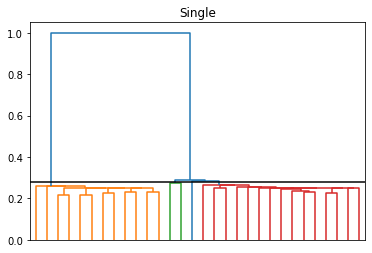
\includegraphics[width=.3\textwidth]{Immagini/GeraSingle.png}
\caption{Cluster gerarchici ottenuti con i metodi \textit{Complete}, \textit{Average} e \textit{Single link}}
\label{fig:clusterGerarchico}

\end{figure}
\noindent I risultati sono stati soddisfacenti solo con il metodo \textit{Complete}. Negli altri casi i cluster risultano sbilanciati, con due cluster contenenti un numero molto basso di oggetti, un cluster eccessivamente grande e un cluster medio. A questo fenomeno vi sono due possibili spiegazioni. \\\\Da una parte, poiché simili risultati sono stati ottenuti anche cercando differenti quantità di cluster, il problema potrebbe essere legato allo stesso dataset: l’alta quantità di rumore avrebbe portato gli algoritmi a costruire delle enormi “catene” incapaci di rilevare validi raggruppamenti per i diversi oggetti. Un'altra possibile spiegazione è che effettivamente sia preferibile avere due grandi cluster, situazione a cui \textit{de facto} hanno portato i due metodi gerarchici. Il clustering generato dal metodo \textit{Single Link} mostra poi un alto valore di \textit{Silhouette}, coerentemente con quanto notato testando il \textit{K-Means} impostando \textit{K} pari a 2. Operare con solo due cluster, però, impedirebbe analisi più dettagliate dei diversi fattori che influenzano \textit{Attrition}.
\\\\I risultati ottenuti dal metodo \textit{Complete}, comunque, non confermano quelli del \textit{K-Means}. La distribuzione degli oggetti è, nel complesso, diversa: nel \textit{K-Means}, ad esempio, avevamo un solo cluster con ampia concentrazione di impiegati con \textit{OverTime}.




\subsection{Conclusioni sul clustering} Dalla nostra analisi l’algoritmo di clustering più efficace per l’analisi del dataset si è dimostrato il \textit{K-Means}. Lo sbilanciamento del dataset e la forte presenza di rumore hanno reso impossibile applicare con risultati significativi i metodi \textit{DBSCAN}, \textit{Gerachico Single-Link} e \textit{Gerarchico Average}. Risultati migliori sono stati ottenuti dal \textit{Gerarchico Complete}, la cui \text{Silhouette} è tuttavia più bassa di quella del \textit{K-Means}.
\vspace{5mm}
\begin{table}[H]
\centering

\begin{tabular}{|l|c|c|}
\hline
\textbf{Algoritmo}                                              & \textbf{Silhouette} \\ \hline
\textit{K-Means}                                                         & 0.397               \\ \hline
\textit{DBSCAN}                                                          & 0.26                \\ \hline
\begin{tabular}[c]{@{}c@{}}Gerarchico\\ (\textit{Complete})\end{tabular} & 0.338               \\ \hline
\end{tabular}
\caption{Tabella riassuntiva sugli algoritmi di clustering applicati e migliori valori della \textit{Silhouette}}
\end{table}
    \section{Classificazione}
In questa parte si è classificato il dataset, al fine di predire in quali casi un lavoratore possa plausibilmente lasciare l’azienda o no (in termini più specifici, quale possa essere il valore della sua \textit{Attrition}). \\
Il metodo di classificazione \textit{Decision Tree} è quello che più di tutti fornisce risultati facilmente leggibili ed è stato quindi scelto per primo. Il carattere fortemente sbilanciato del dataset, in particolare in riferimento all’\textit{Attrition}, ha tuttavia, portato a risultati poco significativi. \\\\
Per ottenere un dataset più bilanciato, abbiamo allora applicato due tecniche di \textit{sampling}: il \textit{Random Undersampling}, che rimuove oggetti della classe maggioritaria (nel nostro caso \textit{Attrition} pari a \textit{No}) e la \textit{Synthetic Minority Oversampling Technique} (\textit{SMOTE}), che genera nuovi oggetti della classe in minoranza (con \textit{Attrition} pari a \textit{Yes}) osservando i preesistenti oggetti più simili.\\\\
Successivamente, abbiamo applicato ulteriori algoritmi di classificazione al dataset, per osservare un possibile aumento dell’accuratezza. Nello specifico, sono stati applicati l’algoritmo \textit{Random Forest} e\textit{ K-Nearest Neighbors} (KNN).

\subsection{Preparazione del dataset}
Il dataset in nostro possesso era già diviso in due parti: il \textit{training set} e il \textit{test set}. Dopo aver proceduto all’eliminazione dei valori mancanti in entrambi (con le procedure di cui abbiamo parlato sopra), abbiamo suddiviso il dataset di \textit{training}: il 70\% è stato destinato effettivamente al \textit{training}, mentre il restante 30\% ha formato il \textit{validation set}, necessario per confrontare fra loro tutti i modelli generati dall’addestramento sul \textit{training} al fine di trovare i parametri ottimali per i classificatori. \\\\Le tecniche di \textit{Oversampling} e \textit{Undersampling} sopra menzionate sono state applicate solo al \textit{training set }in senso stretto.

\subsection{Ottimizzazione dei parametri}
Per quanto riguarda i metodi di \textit{Decision Tree}, l’ottimizzazione dei parametri è stata eseguita applicando l’algoritmo di\textit{ random search} al \textit{training set} originale, sia prima che dopo l’applicazione dello \textit{SMOTE} o del \textit{Random Undersampling}. \\\\L’algoritmo ha addestrato diversi classificatori, testando di volta in volta diverse combinazioni dei parametri\textit{ Max Depth} (profondità massima dell’albero), \textit{Min Sample Split} (numero minimo di oggetti per procedere a una ramificazione) e \textit{Min Sample Leaf} (numero minimo di oggetti per foglia), oltre che possibili misure di impurità (indice di Gini o entropia).
\\\\Nella tabella \ref{tab:TabParametriDecisionTree} riportiamo ciascun parametro dei vari modelli e i relativi risultati: l’accuratezza, il punteggio F1 medio (ovvero, la media della media armonica di \textit{precision} e \textit{recall} per i due valori di \textit{Attrition}) e la curva di ROC (rapporto fra FP e TP). Tali risultati sono riportati sia per il \textit{training set} che per il \textit{validation set}.
\begin{table}[H]
\centering
\resizebox{0.99\textwidth}{!}{
\begin{tabular}{|l|S|S|S|S|S|S|}
\hline
            & \textbf{{Modello 1} }     & \textbf{{Modello 2}}      & \textbf{{Modello 3}}      & \textbf{{Modello 4}}      & \textbf{{Modello 5}}      & \textbf{{Modello 6} }     \\\hline
\textbf{Sampling}     & {Nessuno}     & {Nessuno}     & {\textit{SMOTE}}       & {\textit{SMOTE}}       &\begin{tabular}[c]{@{}c@{}}\textit{Random}\\ \textit{Undersampling}\end{tabular}  & \begin{tabular}[c]{@{}c@{}}\textit{Random}\\ \textit{Undersampling}\end{tabular}   \\
\hline
\textbf{Criterion}    & Gini        & Gini        & {Entropia}    & Gini        & Gini        & Gini        \\ 
\hline
\textbf{Min Sample Split} & 29          & 15          & 31          & 4           & 6           & 23           \\
\hline
\textbf{Min Sample Leaf } & 34          & 25          & 12          & 5           & 9           & 5            \\\hline
\textbf{Max Depth}    & 4           & 12          & 17          & 13          & 17          & 4              \\\hline
\textbf{Training Accuracy}      & 0,851388889 & 0,854166667 & 0,894648829 & 0,931438127 & 0,848360656 & 0,790983607       \\\hline
\textbf{Training F1-Score}  & 1,23507305  & 1,34876709  & 1,78861433  & 1,86287012  & 1,6964715   & 1,58038138                  \\  \hline     
\textbf{Training AUC-ROC}    & 0,594097812 & 0,644703657 & 0,894648829 & 0,931438127 & 0,848360656 & 0,790983607                    \\       \hline   
\textbf{Validation Accuracy}      & 0,844660194 & 0,851132686 & 0,815533981 & 0,763754045 & 0,692556634 & 0,724919094                            \\\hline
\textbf{Validation F1-Score} & 1,11397849  & 1,23989305  & 1,17272962  & 1,17489987  & 1,18883071  & 1,26164874                          \\\hline
\textbf{Validation AUC-ROC}      & 0,553801257 & 0,596041604 & 0,574640826 & 0,589531577 & 0,654108051 & 0,696572882              \\
\hline
\end{tabular}
}
\caption{Parametri, accuratezza, \textit{F1-score} e \textit{AUC-ROC} risultanti dalla \textit{RandomGridSearch} con diverse tecniche di \textit{sampling}}
\label{tab:TabParametriDecisionTree}
\end{table}
\noindent Nei modelli generati dall’algoritmo \textit{Decision Tree}, in media i risultati ottenuti con il \textit{training set} originale hanno valori di accuratezza di 85\% (Modelli 1 e 2). Si è notato un sensibile miglioramento applicando al \textit{training set} lo \textit{SMOTE} (Modelli 3 e 4). Con il \textit{Random Undersampling} non si sono ottenuti invece miglioramenti (Modello 5) e, in taluni casi (Modello 6), si è anzi constatata una diminuzione dell’accuratezza.\\\\
In tutti i modelli addestrati con \textit{SMOTE} o \textit{Random Undersampling} si nota una diminuzione dell’accuratezza sul \textit{validation set}. In fase di test i risultati dell’accuratezza (misurata sia tramite \textit{cross validation} impostata a 10, sia tramite \textit{accuracy score}) hanno confermato questo fenomeno: i modelli ottenuti con tecniche di \textit{sampling} soffrono così di \textit{overfitting}.
\begin{figure}[H]
	\centering
	\subfloat[] 
	{
		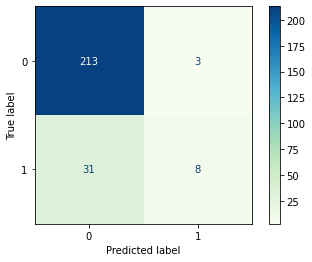
\includegraphics[width=.40\textwidth]{Immagini/MatriceM1.png}
		\label{MatriceM2}
	}
	\quad
	\subfloat[]
	{
		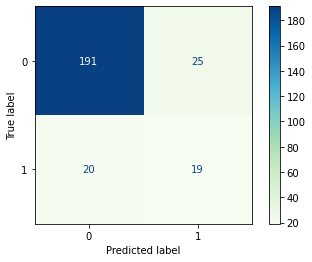
\includegraphics[width=.40\textwidth]{Immagini/MatriceM4.png}
		\label{MatriceM4}
    }
    \caption{Matrici di confusione ottenute applicando sul \textit{test set} il (a) \textit{Modello 1} e (b)\textit{ Modello 4}. Si può notare la difficoltà dei modelli nel riconoscimento corretto dei dipendenti con \textit{Attrition = 1}, ovvero i lavoratori che abbandonano la IBM.}
	\label{MatriciM1M4}
\end{figure}
\begin{figure}[H]
    \centering
    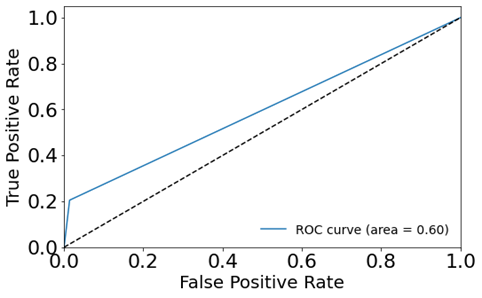
\includegraphics[width=0.45\textwidth]{Immagini/ROCM1.png}
    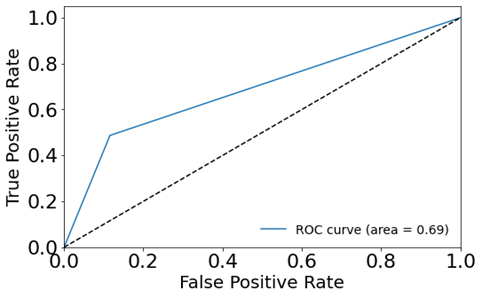
\includegraphics[width=0.45\textwidth]{Immagini/ROCM4.png}
    \caption{Differenti curve di ROC: Modello 1, Modello 4}
    \label{fig:ROC}
\end{figure}
   
\subsection{Altri modelli decisionali}
\begin{wraptable}{r}{70mm}
\centering
\vspace{-1.2cm}
\small
    \begin{tabular}{|c|S|S|}
        \hline
        K & \multicolumn{1}{c|}{\textbf{\begin{tabular}[c]{@{}c@{}}Accuratezza \\ train\end{tabular}}} & \multicolumn{1}{c|}{\textbf{\begin{tabular}[c]{@{}c@{}}Accuratezza \\ con SMOTE\end{tabular}}}\\ \hline
        1 & 0.7424804873405673 & 0.7567086834733894 \\ \hline
        2&0.8085760517799352&  0.7516176470588236 \\\hline
        3&0.7862364363221015&  0.7308263305322129 \\\hline
        4&0.8221682847896441& 0.7308263305322129\\\hline
        5&0.801770416904626&  0.7132703081232493\\\hline
        6&0.8241100323624595&  0.6973879551820729\\ \hline
        7&0.8124595469255663& 0.6923879551820729\\ \hline
        8&0.8279840091376356& 0.6882072829131654\\ \hline
        9&0.8241005139920045& 0.6731442577030813\\ \hline
        10&0.830906148867314& 0.6839705882352941\\ \hline
        11&0.8289644012944983& 0.6781652661064427\\ \hline
    \end{tabular}\setlength{\belowcaptionskip}{-20pt}
    \caption{Accuratezze di diversi KNN con diversi valori di K e \textit{training set}}
\end{wraptable}  

Come detto, sono stai poi applicati altri due algoritmi di classificazione. Il \textit{KNN}, basato sull’osservazione dei valori simili più vicini, ha richiesto lo \textit{scaling} delle varie \textit{\textit{feature}} del dataset. I valori migliori sono stati ottenuti impostando \textit{K} pari a 11 per il \textit{training set} originario e pari a 3 per quello espanso con lo \textit{SMOTE}. Tuttavia, sono risultati in linea con quelli degli alberi decisionali.
\\\\Risultati migliori sono stati invece generati dall’algoritmo \textit{Random Forest}, impostato per generare 100 diversi alberi. Come per gli alberi decisionali, le combinazioni migliori dei parametri sono stati impostate con l’ausilio del \textit{random search}.
\\\\Nella tabella \ref{RandomForest} vengono presentati i risultati ottenuti e una comparazione con due dei metodi ottenuti con gli alberi decisionali.

\begin{table}[H]
\vspace{1em}
\small
\centering
\begin{tabular}{|l|S|S|}
\hline
                          & \textbf{\begin{tabular}[c]{@{}c@{}}Modello \\ Random Forest 1\end{tabular}} & \textbf{\begin{tabular}[c]{@{}c@{}}Modello \\ Random Forest 2\end{tabular}} \\ \hline
\textbf{Sampling}         & {Nessuno}                                                                     & {SMOTE}                                                                       \\ \hline
\textbf{Criterion}        & {Gini, Gini, Gini}                                                            & {Entropia, Gini, Entropia}                                                    \\ \hline
\textbf{Min Sample Split} & {5, 5, 5}                                                                     & {5, 10, 20}                                                                   \\ \hline
\textbf{Min Sample Leaf}  & {1, 1, 5}                                                                     & {1, 1, 1}                                                                     \\ \hline
\textbf{Max Depth}        & {26, 14, 8}                                                                   & {27, 32, 19}                                                                  \\ \hline
\textbf{Train Accuracy}           & 0,973611111                                                                 & 0,987458                                                                    \\ \hline
\textbf{Train F1-Score}    & 1,8999177                                                                   & 1,974913                                                                    \\ \hline
\textbf{Train AUC-ROC}        & 0,922131148                                                                 & 0,987458                                                                    \\ \hline
\textbf{Validation Accuracy}          & 0,851132686                                                                 & 0,847896                                                                    \\ \hline
\textbf{Validation F1-Score}   & 1,23989305                                                                  & 1,286777                                                                    \\ \hline
\textbf{Validation AUC-ROC}          & 0,596041604                                                                 & 0,617106                                                                    \\ \hline
\end{tabular}
\caption{Modelli \textit{Random forest} (con i primi tre alberi) addestrati sul \textit{training set} e sul \textit{training set} su cui è stato applicato lo SMOTE}
\label{RandomForest}
\end{table}

\begin{table}[H]
\resizebox{0.99\textwidth}{!}{
\begin{tabular}{|c|c|c|c|c|}
\hline
                               & \textbf{Modello 1} & \textbf{Modello 4} & \textbf{\begin{tabular}[c]{@{}c@{}}Modello 1 Random\\ Forest\end{tabular}} & \textbf{\begin{tabular}[c]{@{}c@{}}Modello 2 Random \\ Forest (SMOTE)\end{tabular}} \\ \hline
\textbf{Training accuracy}     & 0,851            & 0,931            & 0,973                                                                    & 0,987                                                                             \\ \hline
\textbf{Validation accuracy}   & 0,844            & 0,763            & 0,851                                                                    & 0,847                                                                             \\ \hline
\textbf{Test Accuracy}         & 0.86             & 0.82             & 0.96                                                                     & 0.97                                                                              \\ \hline
\textbf{Cross-validation = 10} & 0.83             & 0.85             & 0.85                                                                     & 0.90                                                                              \\ \hline
\end{tabular}}
\caption{Confronto tra le accuratezze registrate con diversi modelli e diverse composizioni del \textit{training set}}
\end{table}
\noindent I risultati ottenuti sul \textit{training set}, sia per il dataset originario che per quello espanso, sono sensibilmente migliori di quelli offerti dagli alberi decisionali. Si nota anche qui tuttavia una diminuzione con il \textit{validation set}.
Con il \textit{test set}, invece, i due modelli si dimostrano particolarmente efficaci. In particolare il secondo, ottenuto con lo \textit{SMOTE}, ha fornito risultati estremamente positivi, anche osservando la curva di ROC.
\begin{figure}[H]
    \centering
    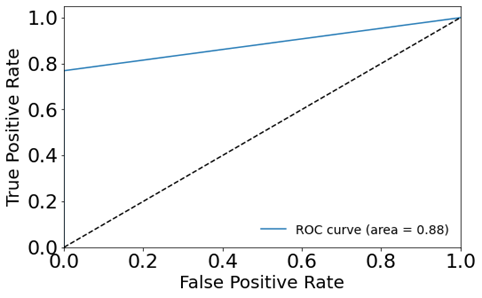
\includegraphics[width=0.45\textwidth]{Immagini/ROCR1.png}
    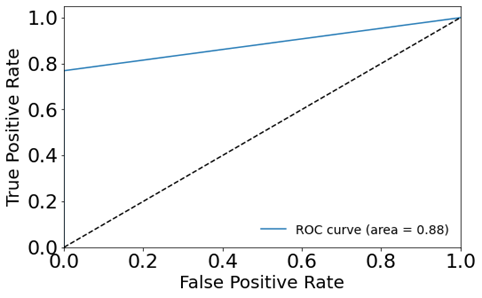
\includegraphics[width=0.45\textwidth]{Immagini/ROCR2.png}
    \caption{Differenti curve di ROC: Random Forest 1, Random Forest 2}
    \label{fig:ROC2}
\end{figure}
% \begin{figure}[H]
% 	\centering
% 	\subfloat[Curva di ROC ottenuta con random forest e addestramento su training set] 
% 	{
% 		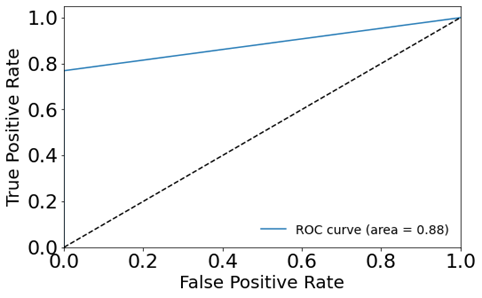
\includegraphics[width=.45\textwidth]{Immagini/ROCR1.png}
% 		\label{ROCRandomForest1}
% 	}
% 	\quad
% 	\subfloat[Curva di ROC ottenuta con random forest e addestramento su training set con SMOTE]
% 	{
% 		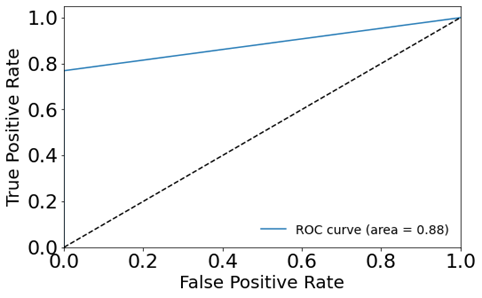
\includegraphics[width=.45\textwidth]{Immagini/ROCR2.png}
% 		\label{ROCRandomForest2}
%     }
% 	\label{ROCRandomForest}
% \end{figure}
Di seguito, il primo albero generato dal modello Random Forest 2.
\begin{figure}[H]
    \centering
    \small
    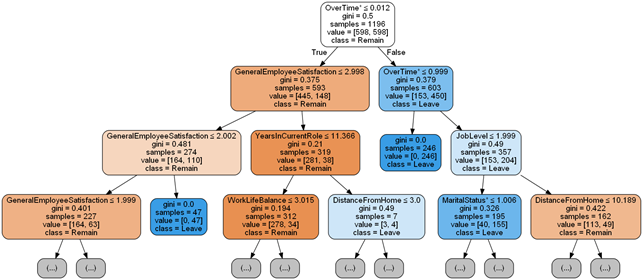
\includegraphics[scale=0.9]{Immagini/alberoRandomForest.png}
    \caption{Albero generato dall'algoritmo \textit{Random Forest}}
    \label{fig:alberoRandomForest}
\end{figure}
\noindent Dall’analisi dell’albero presentato, e dai pesi assegnati da ciascuno dei classificatori addestrati alle diverse \textit{\textit{feature}}, si rileva l’importanza di quattro parametri particolarmente rilevanti per individuare l'\textit{Attrition}: \textit{OverTime}, \textit{JobLevel}, \textit{DistanceFromHome} e \textit{GeneralEmployeeSatisfaction} (i primi tre da noi già utilizzati per il clustering). Meno rilevanti sono, ad esempio, \textit{Gender} e \textit{Age}. 
\\\\Nel caso specifico sopra, si nota, ad esempio, che i lavoratori con basso \textit{OverTime} tendono a rimanere in azienda. Maggiori valori di \textit{OverTime} portano invece all’abbandono dell’azienda, con l’eccezione di alcuni casi determinati da \textit{JobLevel} e \textit{DistanceFromHome}.
\\\\Ulteriori analisi richiederebbero una lettura dell’albero a una maggiore profondità: tuttavia, è da ricordare che quello sopra proposto è soltanto uno dei 100 alberi del \textit{Random Forest}.
\subsection{Conclusioni sulla classificazione}
In generale sono stati notati problemi legati alla natura estremamente sbilanciata del dataset, con una predominanza di oggetti con \textit{Attrition} pari a \textit{No}, che non hanno permesso ai classificatori di riconoscere correttamente i possibili lavoratori che abbandonano l’azienda. \\\\Risultati migliori sono stati ottenuti sul \textit{training set} con l’applicazione del metodo \textit{SMOTE}. Tali modelli non sono comunque risultati adeguati per il \textit{test set} (e il \textit{validation set}), soffrendo di \textit{overfitting}. Il problema si è presentato anche con il classificatore \textit{KNN}, mentre il \textit{Random Forest} ha costituito una valida soluzione, in quanto è un algoritmo nato con lo scopo di evitare le problematiche di \textit{overfitting} che affliggono i tradizionali classificatori basati su alberi di decisione. %applicando un diverso albero decisione a diverse sezioni dal dataset.


    \section{Association Rules}
Questa sezione è dedicata all'\textit{Association Rules Mining}: dopo una prima fase di \textit{data preparation} abbiamo estratto gli \textit{itemset} più frequenti e da questi, attraverso la funzione \textit{Apriori}, ottenuto le regole di associazione. Il nostro obiettivo era quello di trovare delle regole con le quali sostituire i \textit{missing values} presenti nel dataset e costruire un modello predittivo di \textit{Attrition}, la nostra \textit{target variable}.

\subsection{Preparazione dei dati}
Per l'esecuzione delle regole di associazione i dati sono stati preparati come discusso nella sezione di \textit{Data Understanding}, senza però sostituire i \textit{missing values}. Gli attributi quantitativi (\textit{Age} e \textit{MonthlyIncome}) sono stati poi discretizzati nei seguenti intervalli stabiliti osservando i grafici generati con il metodo \textit{KDE} (Fig.\ref{AR}): per \textit{Age} (18.0, 40.0], (40.0, 48.0], (48.0, 62.0], mentre per \textit{MonthlyIncome} (1009.0, 4000.0], (4000.0, 8000.0], (8000.0, 11416.0].
\begin{figure}[H]
	\centering
	\subfloat[] 
	{
		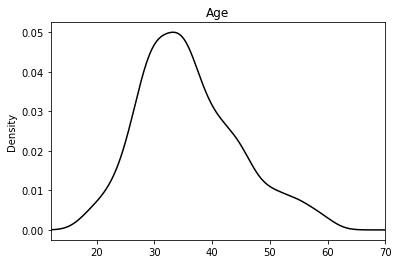
\includegraphics[width=.43\textwidth]{Immagini/kde_Age.png}
		\label{kde_Age}
	}
	\quad
	\subfloat[]
	{
		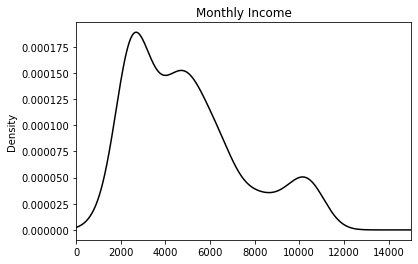
\includegraphics[width =.45\textwidth]{Immagini/kde_MI.png}
		\label{kde_MI}
    }
	\caption{Kernel Density Estimation di Age e MonthlyIncome}
	\label{AR}
\end{figure}
\subsection{\textit{Frequent Itemset}}
Ai dati preparati abbiamo applicato l'algoritmo \textit{Apriori}, con \textit{support} 10\% e lunghezza minima dell'\textit{itemset} 1, per ottenere i \textit{frequent}, i \textit{closed} e i \textit{maximal itemset}. In totale abbiamo ottenuto 431 \textit{frequent} e \textit{closed itemset} e 148 \textit{maximal itemset}. Nelle tabelle Tab. \ref{FrequentItemsets} e Tab. \ref{Maximal Itemsets} abbiamo riportato solo gli itemset con alti valori di \textit{support} (i \textit{frequent itemset} e i \textit{closed itemset} sono identici, e sono stati quindi inseriti nella stessa tabella). L'analisi dei \textit{frequent itemset} evidenzia nuovamente, come già descritto nel \textit{Data Understanding}, che la maggior parte dei lavoratori IBM sono uomini con età compresa tra 18 e 40 anni che possiedono un alto livello di soddisfazione lavorativa e personale e che, dunque, tendono a non licenziarsi. 
\begin{table}[H]
\vspace{3mm}
\centering
\resizebox{.99\textwidth}{!}{
\begin{tabular}{ |p{2cm}|p{10cm}|}
\hline
 \textbf{Support} & \textbf{Frequent-Closed itemsets} \\
 \hline
\textbf{80\% - 90\%}& \textbf{1)} \{Attrition: No\} (\textit{supp} = 0.83)\\
\hline
\textbf{70\% - 80\%}& \textbf{2)} \{OverTime: No\} (\textit{supp} = 0.70)\\
\hline
\textbf{60\% - 70\%}& \textbf{3)} \{OverTime: No, Attrition: No\} (\textit{supp} = 0.63)\\
& \textbf{4)} \{Age: (18.0, 40.0]\} (\textit{supp} = 0.61)\\
& \textbf{5)} \{WorkLifeBalance: High\} (\textit{supp} = 0.60)\\
\hline
\textbf{50\% - 60\%}& \textbf{6)} \{Gender: Male\} (\textit{supp} = 0.57) \\
& \textbf{7)} \{GeneralEmployeeSatisfaction: High\} (\textit{supp} = 0.53)\\
& \textbf{8)} \{WorkLifeBalance: High, Attrition: No\} (\textit{supp} = 0.51)\\
& \textbf{9)} \{Age: (18.0, 40.0], Attrition: No\} (\textit{supp} = 0.50)\\
\hline
\end{tabular}}
\caption{\textit{\textit{Frequent} e \textit{Closed itemset} con un valore di \textit{support} $>$ 50\%}}
\label{FrequentItemsets}
\end{table}
\begin{table}
\centering
\small
\begin{tabular}{ |p{2cm}|p{10cm}|}
\hline
 \textbf{Support} & \textbf{Maximal itemsets} \\
 \hline
\textbf{15\%}& \textbf{1)} \{JobLevel: Low, WorkLifeBalance: High, OverTime: No, Attrition: No\}\\
& \textbf{2)} \{JobLevel: Low, Age: (18.0, 40.0], OverTime: No, Attrition: No\}\\
\hline
\textbf{14\%}& \textbf{3)} \{JobLevel: Very Low, WorkLifeBalance: High, OverTime: No, Attrition: No\}\\
& \textbf{4)} \{Gender: Male, WorkLifeBalance: High, Age: (18.0, 40.0], OverTime: No, Attrition: No\}\\
& \textbf{5)} \{MonthlyIncome: (1009.0, 4000.0], Age: (18.0, 40.0], OverTime: No, Attrition: No\}\\
& \textbf{6)} \{JobLevel: Low, Gender: Male, Overtime: No, Attrition: No\}\\
& \textbf{7)} \{Gender: Female, WorkLifeBalance: High, OverTime: No, Attrition: No\}\\
& \textbf{8)} \{WorkLifeBalance: Medium, Overtime: No, Attrition: No\}\\
& \textbf{9)} \{JobLevel: Very Low, Age: (18.0, 40.0], OverTime: No, Attrition: No\}\\
\hline
\end{tabular}
\caption{\textit{Maximal itemsets ottenuti con min\_support = 0.10}}
\label{Maximal Itemsets}
\end{table}
\subsection{Association Rules}
Dai \textit{frequent itemset} ottenuti abbiamo estratto le regole di associazione impostando una \textit{min\_confidence} del 60\% (regole con \textit{confidence} più bassa, vere cioè meno del 60\% delle volte, sono poco informative). Abbiamo così ottenuto 965 regole. Alcune di esse, come si può notare dai grafici seguenti (Fig. \ref{Confidence}), presentano una \textit{confidence} compresa tra 80\% e 90\%. 
\begin{figure}[H]
	\centering
	\subfloat[] 
	{
		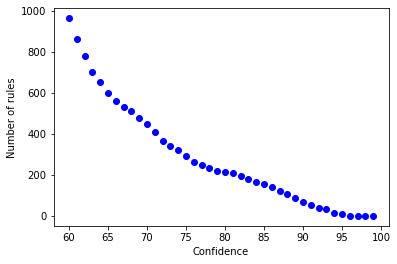
\includegraphics[width=.45\textwidth]{Immagini/confidence.png}
		\label{Conf}
	}
	\quad
	\subfloat[]
	{
		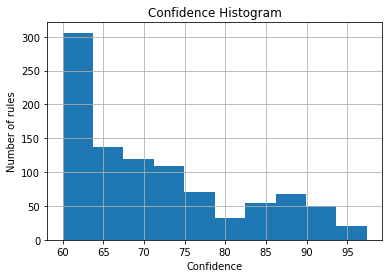
\includegraphics[width =.45\textwidth]{Immagini/hist_conf.png}
		\label{Conf_hist}
    }
	\caption{Distribuzione del numero di regole in base ai valori di \textit{confidence}}
	\label{Confidence}
\end{figure}
\noindent 
Per quanto riguarda il \textit{lift} (Fig. \ref{lift}), la sua distribuzione è sbilanciata verso il valore di 1: vi sono, quindi, molte regole i cui elementi sono associati tra loro in maniera casuale. Solo un piccolissimo numero di regole ha lift compreso tra 1.6 e 1.9. 
\begin{figure}[H]
    \centering
    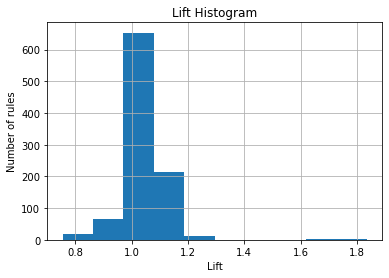
\includegraphics[scale=0.5]{Immagini/lift.png}
    \caption{Distribuzione del numero di regole in base ai valori di lift}
    \label{lift}
\end{figure}
\noindent Delle 965 regole abbiamo selezionato le più informative. Per il principio di anti-monotonicità su cui si basa l'algoritmo \textit{Apriori}, riportiamo successivamente solo 8 regole, ordinate secondo il parametro di lift, generate da diversi itemset.
\begin{table}[H]
\centering
\small
\begin{tabular}{|p{15cm}|}
\hline
 \textbf{Association Rules} \\
 \hline
\{Attrition: Yes, Age: (18.0, 40.0]\} $=>$ JobLevel: Very Low (\textit{conf} = 0.71) (\textit{lift} = 1.83)\\
\hline
\{MonthlyIncome: (1009.0, 4000.0], Marital Status: Married\} $=>$ Age: (18.0, 40.0] (\textit{conf} = 0.74) (\textit{lift} = 1.21)\\
\hline
\{JobLevel: Very Low, Gender: Male, WorkLifeBalance: High, Attrition: No\} $=>$ OverTime: No (\textit{conf} = 0.86) (\textit{lift} = 1.21)\\
\hline
\{MonthlyIncome: (1009.0, 4000.0], JobLevel: Very Low\} $=>$ Age: (18.0, 40.0] (\textit{conf} = 0.74) (\textit{lift} = 1.21)\\
\hline
 \{OverTime: Yes, Gender: Male, Attrition: No\} $=>$ GeneralEmployeeSatisfaction: High (\textit{conf} = 1.83) (\textit{lift} = 0.64)\\
\hline
\{JobLevel: Low, GeneralEmployeeSatisfaction: High, Age: (18.0, 40.0]\} $=>$ Attrition: No (\textit{conf} = 0.97) (\textit{lift} = 1.17)\\
\hline
\{Gender: Male, WorkLifeBalance: High, Age: (18.0, 40.0], OverTime: No\} $=>$ Attrition: No (\textit{conf} = 0.95) (\textit{lift} = 1.15)\\
\hline
\{GeneralEmployeeSatisfaction: Medium, MonthlyIncome: (1009.0, 4000.0]\} $=>$ Gender: Male (\textit{conf} = 0.64) (\textit{lift} = 1.12)\\
\hline
\end{tabular}
\caption{\textit{Association Rules più interessanti, ordinate per valore di lift}}
\label{ARinteressanti}
\end{table}
\noindent Osservando queste regole possiamo affermare che circa il 96\% dei lavoratori IBM non si licenzia e nell'86\% dei casi non fa straordinari. Con probabilità del 75\%, i dipendenti hanno età compresa tra 18 e 40 anni e sono uomini nel 64\% dei casi. La quinta regola, infine, evidenzia che nel 64\% dei casi i lavoratori sono molto soddisfatti del loro lavoro (dimostrando che la nuova \textit{feature} da noi creata (\textit{GeneralEmployeeSatisfaction}) è risultata utile nelle analisi). 
\subsection{Sostituzione dei \textit{missing values}}
Dopo aver estratto le regole più interessanti, abbiamo sostituito i valori mancanti di \textit{Age}, \textit{MonthlyIncome} e \textit{Gender}.
\begin{itemize}
\item \textit{Age} presentava 168 \textit{missing values} e con le regole estratte (con \textit{confidence} compresa tra 60\% e 75\%) siamo riusciti a sostituirne 89 con il valore (18.0, 40.0]. Gli altri intervalli d'età presentavano una \textit{confidence} minore nel 60\% e non sono stati considerati validi per la sostituzione;
\item \textit{MonthlyIncome} aveva 213 \textit{missing values} che non siamo riusciti a sostituire in quanto le prime regole utili per la sostituzione hanno tutte una \textit{confidence} del 40\%;
\item \textit{Gender} aveva 51 \textit{missing values} e con le regole estratte (con \textit{confidence} compresa tra 60\% e 64\%) siamo riusciti a sostituirne 40 con il valore \textit{Male}. Per il valore di \textit{Female} non abbiamo trovato regole con una \textit{confidence} maggiore del 60\%.
\end{itemize}
\subsection{Predizione della \textit{target variable}}
Abbiamo usato le regole estratte per costruire un modello predittivo per la nostra \textit{target variable}. L'accuratezza del modello è del 94\%. Sebbene possa apparire un ottimo risultato, il modello assegna sempre e solo il valore di \textit{Attrition: No} dal momento che non vi sono regole con \textit{confidence} maggiore del 60\% che hanno come conseguenza \textit{Attrition: Yes}.\\\\
Tuttavia abbiamo deciso di rilanciare il modello includendo la prima regola che comprendesse \textit{Attrition: Yes}, che presenta \textit{confidence} pari a 57\%, un valore di poco minore di 60\%. La nuova accuratezza è risultata dell'82\%, ancora un valore alto, ma a causa del forte sbilanciamento dei dati il modello ha continuato ad associare solo il valore di \textit{Attrition: No}.






    \section{Conclusioni}
Riassumendo, l’analisi del dataset si è ripetutamente scontrata con il suo alto sbilanciamento e la presenza di dati mancanti o corrotti, già rilevati nella fase di \textit{Data understanding}.\\\\
Nella fase di \textit{Data preparation} si è cercato limitare il problema, rimuovendo i parametri giudicati poco utili, stimando i possibili valori mancanti nelle varie \textit{feature} e generando due nuove \textit{feature} \textit{ad hoc}, che si sono in seguito rivelate utili. Nel complesso, i 1176 oggetti descritti da 33 attributi sono stati ridotti a 1029 oggetti descritti da 13 attributi.\\\\
Il clustering dei dati è risultato tuttavia comunque problematico per il generale sbilanciamento degli oggetti con \textit{Attrition} pari \textit{No} e la presenza di rumore. Dei vari modelli testati, solo il \textit{K-Means} ha portato a dei buoni risultati. \\\\
Successivamente si è proceduto alla classificazione dei dati. Nuovamente, le problematiche descritte sopra hanno portato gli algoritmi di \textit{Decision tree} e \textit{KNN} a generare risultati poco soddisfacenti. Di contro, il metodo \textit{Random forest}, accompagnato da un \textit{oversampling} del dataset, è risultato efficace e ha permesso di comprendere quali attributi potessero maggiormente determinare l’\textit{Attrition}: \textit{OverTime}, \textit{JobLevel}, \textit{GeneralEmployeeSatisfaction} e \textit{DistanceFromHome}. È stato inoltre addestrato un modello per la predizione della \textit{target variable}, che, tuttavia, non ha fornito risultati accurati. \\\\
Eventuali sviluppi futuri potrebbero vedere l’applicazione di altri algoritmi o in alternativa l’ampliamento dell’attuale dataset, per avere una prospettiva meno sbilanciata dei lavoratori IBM, permettendo,  anche soltanto con le metodologie testate in questo \textit{paper}, di ottenere risultati più accurati.



    
\end{document}
